% Copyright (C) 2024 Songbingzhi628. This work is licensed under Creative Commons Attribution-NonCommercial-ShareAlike 4.0 International License.
% Email: 13012057210@163.com

\ChDecl{Ch4O}{4}{}%\orMode{\hLk{4O5}{5}\;\;\hLk{4O6}{6}\;\;\hLk{4O7}{7}\;\;\hLk{4O8}{8}\;\;\hLk{4O9}{9}\;\;\hLk{4O10}{10}\;\;\hLk{4O11}{11}\;\;|\;\;\hLk{4O4e2}{4E:\;\;2}\;\;\hLk{4O4e3}{3}\;\;\hLk{4O4e13}{13}}{[1]: (4E 2), 5; [2]: 6, 7, 8, 11; [3]: 9, 10, (4E 13).}

\vspace{3pt}

\Anchor{4OT1}\BulletPointX\TipsN{1}\,\,\,{\tgsl Supp $p\in\PoF{n}$ has at least $n+1$ disti zeros. Then by the ctrapos of [4.12], $\deg p<0\Rightarrow p=0.$}\TextB{}
\Or We show if $p\in\PoFi{}$ has at least $m$ disti zeros, then either $p=0$ or $\deg p\geqslant m.$\TextB{}
If $p=0$ then done. If not, then supp $p$ has exactly $m$ disti zeros $\lambda_1,\dots,\lambda_m.$\TextB{}
Becs $\exists\,!\,\alpha_i\geqslant 1,q\in\PoFi,$ and $q\neq 0,$ suth $p\Par{z}=\Sbra{\Par{z-\lambda_1}{^{\alpha_1}}\cdots\Par{z-\lambda_m}{^{\alpha_m}}}q\Par{z}.$\PfEnd\vspace{2pt}
\BulletPointX\AComm {\tgsl\NOTICE that by [4.17], some term of the poly factoriz might not be in the form $\Par{x-\lambda_k}{^{\alpha_k}}.$}\vspace{-2pt}
\SepLine

\Anchor{4ON4.7}\BulletPointX\NoteFor{[4.7]} {\tgsl the uniqnes of coeffs of polys} \hfill[{\tgsc Another proof}]\TextB{\vspace{2pt}}
If a poly had two different sets of coeffs, then
subtracting the two exprs\TextB{}
would give a poly with some non0 coeffs but infily many zeros. By {\TIPS}.\PfEnd\vspace{-3pt}
\SepLine

\Anchor{4ON4.8}\BulletPointX\NoteFor{[4.8]} {\tgsl div algo for polys} \hfill[{\tgsc Another proof}]\TextB{\vspace{-11pt}}
Supp $\deg p\geqslant \deg s$. Then $\FontLarge\BigPar{\FontNorm\underbrace{1, z,\dots, z^{\deg s-1}}_{\text{of\,len}\,\deg s},\overbrace{s,zs,\cdots,z^{\deg p-\deg s}s}^{\text{of\,len}\,\SmallPar{\deg p\,-\,\deg s\,+\,1}}\FontLarge}$ is a bss of $\PoF{\deg p}.$\TextB{\vspace{-7pt}}
Becs $q\in\PoFi,\exists\,!\,a_i,b_j\in\Fbb,$\TextB{}
$q=a_0+a_1 z+\dots+a_{\deg s-1}z^{\deg s-1}+ b_0 s+b_1 zs +\dots+ b_{\deg p-\deg s}z^{\deg p-\deg s}s$\TextB{}
$\Blind{q}=\underbrace{a_0+a_1 z+\dots+a_{\deg s-1}z^{\deg s-1}}_{r}+s\underbrace{\XPar{b_0+b_1 z +\dots+ b_{\deg p-\deg s}z^{\deg p-\deg s}}}_{q}.$ Note that $r,q$ are uniq.\PfEnd[-16pt]
\SepLine

\Anchor{4ON4.11}\BulletPointX\NoteFor{[4.11]}\;\;{\tgsl each zero of a poly corres to a deg-one factor;}\hfill[{\tgsc Another proof}]\TextB{\vspace{2pt}}
First supp $p\Par{\lambda}=0.$ Write $p\Par{z}=a_0+a_1 z+\dots+a_m z^m,\exists\,!\,a_0,a_1,\dots,a_m\in\Fbb$ for all $z\in\Fbb.$\vspace{2pt}\TextB{}
Then $p\Par{z}=p\Par{z}-p\Par{\lambda}=a_1\Par{z-\lambda}+\dots+a_m\Par{z^m-\lambda^m}$ for all $z\in\Fbb.$\vspace{2pt}\TextB{}
Hence $\forall k\in\Bra{1,\dots,m},z^k-\lambda^k=\Par{z-\lambda}\Par{ z^{k-1}\lambda^0+ z^{k-2}\lambda^1+\dots+z^{k-\SmallPar{j+1}}\lambda^j+\dots+z\lambda^{k-2}+z^0\lambda^{k-1}}.$\vspace{4pt}\TextB{}
Thus $p\Par{z}=\sum_{j=1}^m a_j \Par{z-\lambda}\sum_{i=1}^k \lambda^{i-1}z^{k-i}=\Par{z-\lambda}\sum_{j=1}^m a_j\sum_{i=1}^k \lambda^{i-1}z^{k-i}=\Par{z-\lambda}q\Par{z}.$\PfEnd
\SepLine

%\BulletPointX\NoteFor{[4.13]}\;\;{\tgsl Every nonC poly with complex coeffs has a zero in $\Cbb$.} \vspace{2pt}\hfill[{\tgsc Another proof}]\TextB{}
%For any $w\in\Cbb,k\in\Nbp,$ by polar coordinates, $\exists\,r\geqslant 0,\theta\in\Rbb,r\Par{\cos\theta + \i \sin\theta} = w$.\vspace{2pt}\TextB{}
%By De Moivre' theorem, $w^k=\Sbra{r\Par{\cos\theta +\i\sin \theta}}{^k}=r^k\Par{\cos k\theta + \i \sin k\theta}$.\vspace{2pt}\TextB{}
%Hence $\BigPar{r^{1/k}\Par{\cos\frac{\;\theta\;}{k} +\i\sin\frac{\;\theta\;}{k}}}{^k}=w$. Thus every complex number has a {\tgsl $k^{th}$ root}.\vspace{6pt}\TextB{}
%Supp a nonC $p\in\PoCi$ with highest-order non0 term $c_m z_m.$\vspace{3pt}\TextB{}
%Then $\aMid{p\Par{z}}\rightarrow\infty$ as $\aMid{z}\rightarrow\infty$ \XPar{ becs $\Frac{\aMid{p\Par{z}}}{\aMid{z_m}}\rightarrow\aMid{c_m}$ as $\aMid{z}\rightarrow\infty$ }.\vspace{3pt}\TextB{}
%\vspace{3pt}Thus the continuous function $z\rightarrow\aMid{p\Par{z}}$ has a global min at some point $\zeta\in\Cbb.$\TextB{}
%\vspace{3pt}To show $p\Par{\zeta} = 0$, asum $p\Par{\zeta}\neq 0$. Define $q\in\PoCi$ by $q\Par{z}=\Frac{p\Par{z+\zeta}}{p\Par{\zeta}}.$\TextB{}
%\vspace{3pt}The function $z\rightarrow\aMid{q\Par{z}}$ has a global min value of $1$ at $z = 0$.\TextB{}
%\vspace{3pt}Write $q\Par{z} = 1 + a_k z^k + \dots + a_m z^m$, where $k\in\Nbp$ is the smallest suth $a_k\neq 0$.\TextB{}
%\vspace{3pt}Let $\beta\in\Cbb$ be suth $\beta^k=-\Frac{1}{a_k}$.\TextB{}
%\vspace{4pt}There is a const $c > 1$ so that if
%$t\in \Par{0, 1}$, then $\aMid{q\Par{t\beta}}\leqslant\aMid{1 + a_k t^k\beta^k}+t^{k+1}c = 1 - t^k \Par{1 - tc}$.\TextB{}
%Now letting $t=1/\Par{2c}$, we get $\aMid{q\Par{t\beta}}<1$. Ctradic. Hence $p\Par{\zeta} = 0$, as desired.\PfEnd
%\SepLine

\Anchor{4O4e2}\ProblemBnoor{4E 2}{
	\TextB{Prove if $w,z\in\Cbb,$ then $\aXMid{\aMid{w}-\aMid{z}}\leqslant\aMid{w-z}.$}
}$\aMid{w-z}{^2}=\Par{w-z}\Par{\overline{w}-\overline{z}}=\aMid{w}{^2}+\aMid{z}{^2}-2Re\Par{w\overline{z}}\geqslant\aMid{w}{^2}+\aMid{z}{^2}-2\aMid{w\overline{z}}=\aXMid{\aMid{w}-\aMid{z}}{^2}.$\vspace{2pt}\parSol{}
\Or $\aMid{w}=\aMid{w-z+z}\leqslant\aMid{w-z}+\aMid{z}\Rightarrow \aMid{w}-\aMid{z}\leqslant\aMid{w-z}.$\parSol{}
\Blind{\Or}$\aMid{z}=\aMid{z-w+w}\leqslant\aMid{z-w}+\aMid{w}\Rightarrow \aMid{z}-\aMid{w}\leqslant\aMid{w-z}.$\PfEnd
\SepLine

\ProblemN{\Anchor{4O5}{5}}{
	\TextA{Supp $m\in\Nbb,$ and $z_1,\dots,z_{m+1}$ are disti in $\Fbb,$ and $w_1,\dots,w_{m+1}\in\Fbb.$}
	\TextA{Prove $\exists\,!\,p\in\PoF{m},p\Par{z_k}=w_k$ for each $k\in\Bra{1,\dots, m+1}.$}
}\par\quad
Define $T\in\Lm[\BigPar]{\PoF{m},\Fbb^{m+1}}$ by $Tq=\BigPar{q\Par{z_1},\dots,q\Par{z_m},q\Par{z_{m+1}}}.$\vspace{1pt}\par\quad
Becs $Tq=0\Longleftrightarrow q\Par{z_1}=\dots=q\Par{z_m}=q\Par{z_{m+1}}=0\Longleftrightarrow q=0,$ by {\TIPS}. \;Now $T$ iso. Immed.\PfEnd\vspace{4pt}\quad
\Or Let $p_1=1,\;p_k\Par{z}=\prod_{i=1}^{k-1}\Par{z-z_i}=\Par{z-z_1}\cdots\Par{z-z_{k-1}}$ for each $k\in\Bra{2,\dots,m+1}.$\vspace{1pt}\par\quad
By (2.C.10), $B_p=\Par{p_1,\dots,p_{m+1}}$ is a bss of $\PoF{m}.$ Let $B_e=\Par{e_1,\dots,e_{m+1}}$ be the std bss of $\Fbb^{m+1}.$\vspace{2pt}\par\quad
Now $Tp_1=\Par{1,\dots,1},\;Tp_k=\XPar{\prod_{i=1}^{k-1}\Par{z_1-z_i},\dots,\prod_{i=1}^{k-1}\Par{z_j-z_i},\dots,\prod_{i=1}^{k-1}\Par{z_{m+1}-z_i}};$\vspace{3pt}\par\quad
{\normalsize$\begin{pmatrix}
		1 &\hspace{-6pt} 0 &\hspace{-6pt} 0 &\hspace{-6pt} \cdots &\hspace{-6pt} 0\\[-2pt]
		1 &\hspace{-6pt} A_{2,2} &\hspace{-6pt} 0 &\hspace{-6pt} \cdots &\hspace{-6pt} 0\\[-2pt]
		1 &\hspace{-6pt} A_{3,2} &\hspace{-6pt} A_{3,3} &\hspace{-6pt} \cdots &\hspace{-6pt} 0\\[-2pt]
		\vdots &\hspace{-6pt} \vdots &\hspace{-6pt} \vdots &\hspace{-6pt} \ddots &\hspace{-6pt} \vdots\\[-2pt]
		1 &\hspace{-6pt} A_{m+1,2} &\hspace{-6pt} A_{m+1,3} &\hspace{-6pt} \cdots &\hspace{-6pt} A_{m+1,m+1}
	\end{pmatrix}$}${}=\Mt[\BigPar]{T,B_p,B_e}.$ Where $A_{j,k}=\prod_{i=1}^{k-1}\Par{z_j-z_i}\neq 0$ for all $j> k-1\geqslant 1.$\vspace{-74pt}\par\quad
\hfill And $\prod_{i=1}^{k-1}\Par{z_j-z_i}=0 \Longleftrightarrow j\leqslant k-1,$ becs $z_1,\dots,z_{m+1}$ are disti.\Blind{\quad\qquad}\vspace{30pt}\par\quad
\hfill Now the rows $\Mt{T}$ are liney indep. By (4E 3.C.17) \OR (3.F.32).\Blind{\quad}\PfEnd\vspace{3pt}
\SepLine

%\Anchor{4O4}\ProblemN[]{{4}}{
%	For $m,n\in\Nbp$ with $m\leqslant n,\;\lambda_1,\dots,\lambda_m\in\Fbb,$ let $p\Par{z}=\Par{z-\lambda_1}{^{n-\SmallPar{m-1}}}\Par{z-\lambda_2}\cdots\Par{z-\lambda_m}\Rightarrow\deg p=n.$\TextA{}
%}\SepLine

%\ProblemN{\Anchor{4O2}{2}}{
%	\TextA{Supp $m\in\Nbp$. Is the set $U=\zeroSubs\cup\Bra{p\in\PoFi:\deg p = m}$ a subsp of $\PoFi$?}
%}$x^m,x^m+x^{m-1}\in U$ \,\,but\,\, $\Deg\Sbra{\Par{x^m+x^{m-1}}-\Par{x^m}}\neq m\Rightarrow \Par{x^m+x^{m-1}}-\Par{x^m}\not\in U.$\PfEnd
%\SepLine
%
%\ProblemN{\Anchor{4O3}{3}}{
%	\TextA{Supp $m\in\Nbp$. Is the set $U=\zeroSubs\cup\Bra{p\in\PoFi:2\;\mmid\,\deg p}$ a subsp of $\PoFi$?}
%}$x^2,x^2+x\in U$ \,\,but\,\, $\Deg\Sbra{\Par{x^2+x}-\Par{x^2}}$ is odd and hence $\Par{x^2+x}-\Par{x^2}\not\in U.$\PfEnd
%\SepLine

\ProblemN{\Anchor{4O6}{6}}{
	\TextA{Supp non0 $p\in\PoF{m}$ has deg $m.$ Prove}
	\TextA{[P] $p$ has $m$ disti zeros $\Longleftrightarrow p$ and its deri $p\apostrophe$ have no common zeros. [Q]}
}(a) Supp $p$ of deg $m$ has $m$ disti zeros. By [4.14], $p\Par{z}=c\Par{z-\lambda_1}\cdots\Par{z-\lambda_m}.$\vspace{1pt}\parSol{\Ha}
If $m=0,$ then $p=c\neq 0\Rightarrow p$ has no zeros, and $p\apostrophe=0,$ done.\parSol{\Ha}
If $m=1,$ then $p\Par{z}=c\Par{z-\lambda_1},$ and $p\apostrophe=c$ has no zeros, done.\vspace{1pt}\parSol{\Ha}
For each $j\in\Bra{1,\dots,m}$, let $q_j\Par{z-\lambda_j}=p\Par{z}\Rightarrow q_j\Par{\lambda_j}\neq 0.$\vspace{1pt}\parSol{\Ha}
Now $p\apostrophe\Par{z}=\Par{z-\lambda_j}q_j\apostrophe\Par{z}+q_j\Par{z}\Rightarrow p\apostrophe\Par{\lambda_j}=q_j\Par{\lambda_j}\neq 0.$\vspace{4pt}\parSol{\Ha}
\Or ${}^{\neg}Q\Rightarrow{}{^\neg}P:$ \;Supp $p\Par{z}=\Par{z-\lambda}q\Par{z},\;p\apostrophe\Par{z}=\Par{z-\lambda}r\Par{z}.$\parSol{\Ha}
Becs $p\apostrophe\Par{z}=\Par{z-\lambda}q\apostrophe\Par{z}+q\Par{z}\Rightarrow p\apostrophe\Par{\lambda}=q\Par{\lambda}=0\Rightarrow q\Par{z}=\Par{z-\lambda}s\Par{z}.$\parSol{\Ha}
Now $p\Par{z}=\Par{z-\lambda}{^2}s\Par{z}.$ Hence $p$ has strictly less than $m$ disti zeros.\vspace{4pt}\parSol{}
(b) ${}^{\neg}P\Rightarrow{}{^\neg}Q:$ \;Becs $0\neq p\in\PoF{m}.$ Supp all disti zeros are $\lambda_1,\dots,\lambda_M,$ with $M<m.$\parSol{\Hb}
By Pigeon Hole Principle, $\Par{z-\lambda_k}{^{2}}q\Par{z}=p\Par{z}$ for some $\lambda_k\Rightarrow p\apostrophe\Par{\lambda_k}=0=p\Par{\lambda_k}.$\PfEnd
\SepLine

\ProblemN{\Anchor{4O7}{7}}{
	\TextA{Prove every $p\in\PoRi$ of odd deg has a zero.}
}Using the nota and proof of [4.17]. $\deg p=2M+m$ is odd $\Rightarrow m$ is odd. Hence $\lambda_1$ exis.\PfEnd\vspace{3pt}\parSol{}
\Or Supp $p\in\PoRi$ of odd deg $m.$ Let $p\Par{x}=a_0+a_1 x+\dots+a_m x^m.$\parSol{\vspace{3pt}}
Write $p\Par{x}=x^m\envFontSmall\XPar{${\FontLarge$\frac{a_0}{x^m}$}${}+{}${\FontLarge$\frac{a_1}{x^{m-1}}$}${}+\dots+{}${\FontLarge$\frac{a_{m-1}}{x}$}${}+a_m\envFontSmall}\Rightarrow p\Par{x}$ continuous. Let $\delta=\aMid{a_m}{^{-1}}a_m.$\parSol{\vspace{3pt}}
Then $\lim\limits_{x\rightarrow -\infty}p\Par{x}=-\delta\infty\,;\;\;\lim\limits_{x\rightarrow \infty}p\Par{x}=\delta\infty\Rightarrow p$ has at least one real zero.\PfEnd
\SepLine

\ProblemN{\Anchor{4O8}{8}}{
	\TextA{Supp $p\in\PoRi.$ Define $Tp:\Rbb\rightarrow\Rbb\,$ by $\Par{Tp}\Par{x}={}${\FontNorm$\MathLeftBrace{l}{\Frac{p\Par{x}-p\Par{3}}{x-3}\;$ if $x\neq 3,\\[4pt]p\apostrophe\Par{3}$\hfill if $x=3.}$}\vspace{-10pt}}
	\TextA{Show {\tgnr\large(a)} $Tp\in\PoRi;$ \, {\tgnr\large(b)} $T\in\Lm[\BigPar]{\PoRi}.$\vspace{0pt}}
}\vspace{2pt}\par\quad
(a) For $x\neq 3,T\Par{x^n}={}${\Large$\frac{x^n\,-\,3^n}{x\,-\,3}$}${}=\sum_{i=1}^n 3^{i-1}x^{n-i}.$\vspace{2pt}\par\quad\Ha
For $x=3,T\Par{x^n}=n3^{n-1}=\sum_{i=1}^n 3^{n-1}=\sum_{i=1}^n 3^{i-1}x^{n-i}.$ \,Now each $T\Par{x^n}=\sum_{i=1}^n 3^{i-1}x^{n-i}\in\PoRi{}.$\par\vspace{8pt}\quad
(b) $T\Par{p+\lambda q}\Par{x}={}${\FontSmall$\hMath{l}{\left\{}{\right|}{
		\Frac{\Par{p+\lambda q}\Par{x}-\Par{p+\lambda q}\Par{3}}{x-3},\;$ if $x\neq 3,\\
		\Par{p+\lambda q}\apostrophe\Par{3},$ \hfill if $x=3\Blind{.}
	}$}${}=\Sbra{T\Par{p}+\lambda T\Par{q}}\Par{x}$ for all $x\in\Rbb.$\PfEnd\vspace{16pt}\quad
\Or (a) Becs $\exists\,!\,q\in\PoRi,p\Par{x}-p\Par{3}=\Par{x-3}q\Par{x}.$ For $x\neq 3,\;q\Par{x}={}${\Large\envFontSmall[\footnotesize]\def\SmallPar{\Par}$\frac{p\SmallPar{x}\,-\,p\SmallPar{3}}{x\,-\,3}$}.\par\quad\Ha
\Blind{\Or}$p\apostrophe\Par{x}=\BigPar{p\Par{x}-p\Par{3}}\apostrophe=q\Par{x}+\Par{x-3}q\apostrophe\Par{x}.$ For $x=3,\;p\apostrophe\Par{3}=q\Par{3}.$ Now $Tp=q.$\vspace{4pt}\par\quad
\Blind{\Or}(b) Let $q_k\Par{x}\Par{x-3}=p_k\Par{x}-p_k\Par{3}.$ Now by (a), $Tp_k=q_k.$\par\quad\Hb
\Blind{\Or}Then $\Par{p_1+\lambda p_2}\Par{x}-\Par{p_1+\lambda p_2}\Par{3}=\Par{x-3}\Par{q_1+\lambda q_2}\Par{x}.$ \,By the uniqnes of $q_1+\lambda q_2.$\PfEnd
\SepLine

\ProblemN{\Anchor{4O11}{11}}{
	\TextA{Supp $p\in\PoFi$ with $p\neq 0$. Let $U=\Bra{pq:q\in\PoFi}$.\vspace{1pt}}
	\TextA{{\tgnr\large(a)} Show $\dim\PoFi\XSlash U = \deg p$; \; {\tgnr\large(b)} Find a bss of $\PoFi\XSlash U$.}
}{\tgsl Note that $pq\neq p\circ q,$ see (4E 3.A.10).} \;Let $\deg p=m$ as precond.\par\quad
If $\deg p=0,$ then $U=\PoFi,\PoFi\XSlash U=\Bra{0+U},$ with the uniq bss $\Par{}.$ \;Supp $\deg p\geqslant 1.$\par\vspace{2pt}\quad
(a) Becs $\forall s\in\PoFi,\exists\,!\,r\in\PoF{m-1},q\in\PoFi\Rightarrow\exists\,!\,pq\in U,\;s=\Par{p}q+\Par{r}\Rightarrow\PoFi=U\oplus\PoF{m-1}.$\vspace{0pt}\par\quad\Ha
By \Sbra{3.E {\NOTEFOR} [3.88, 90, 91]} \OR Define $R\Par{s}=r\Rightarrow\null R=U,$ and $R$ surj. Immed.\par\vspace{2pt}\quad
(b) Let $\Par{1,z,\dots,z^{m-1}}$ be a bss of $\PoF{m-1}.$ By (4E 3.E.14) \OR $\tilde{R}{^{-1}}\!:\PoF{m-1}\rightarrow\PoFi{}\XSlash U$, immed.\PfEnd
\SepLine\pagebreak

\ProblemN{\Anchor{4O9}{9}}{
	\TextA{Supp $p\in\PoCi$. Define $q:\Cbb\rightarrow\Cbb\,$ by $q\Par{z} = p\Par{z}\overline{p\Par{\overline z}}$. Prove $q\in\PoRi$.\vspace{1pt}}
}By [4.5], $\overline z{^n}=\overline{z^n}.$ \;For any $f\Par{z}=a_nz^n+\dots+a_1z+a_0,\;\overline{f\Par{\overline{z}}}=\overline{a_n}z^n+\dots+\overline{a_1}z+\overline{a_0}.$\parSol{}
Becs $q\Par{z}=p\Par{z}\overline{p\Par{\overline z}}=\overline{p\Par{\overline z}}p\Par{z}=\overline{q\Par{\overline z}}.$ \;Each $c_k=\overline{c_k}\Rightarrow c_k\in\Rbb.$\PfEnd\vspace{6pt}\parSol{}
\Or Becs $q\Par{z}=p\Par{z}\overline{p\Par{\overline z}}=\sum_{k=0}^{2n}\XPar{{\sum_{i+j=k}c_i\overline{c_j}}}\,z^k.$ For each $k\in\Bra{0,\dots,2n},$\vspace{0pt}\parSol{}
$\overline{\sum_{i+j=k}c_i\overline{c_j}}=\sum_{i+j=k}\overline{c_i\overline{c_j}}=\sum_{i+j=k}{c_j}\overline{c_i}=\sum_{i+j=k}c_i\overline{c_j}\in\Rbb.$\PfEnd
\SepLine

\ProblemN{\Anchor{4O10}{10}}{
	\TextA{Supp disti $x_0,x_1,\dots,x_m\in\Rbb,$ and $p\in\PoC{m}$ suth each $p\Par{x_k}\in\Rbb.$ Prove $p\in\PoRi$.}
}By {\TIPS} and Exe (5), $\exists\,!\,q\in\PoR{m}$ suth $q\Par{x_k}=p\Par{x_k}.$ Hence $p=q.$\PfEnd\vspace{11pt}\quad
\Or Define $q\Par{x}=\sum_{j=0}^m{}${\Large\envFontSmall[\footnotesize]\def\SmallPar{\Par}$\frac{\SmallPar{x\,-\,x_0}\SmallPar{x\,-\,x_1}\,\cdots\,\SmallPar{x\,-\,x_{j-1}}\SmallPar{x\,-\,x_{j+1}}\,\cdots\,\SmallPar{x\,-\,x_m}}{\SmallPar{x_j\,-\,x_0}\SmallPar{x_j\,-\,x_1}\,\cdots\,\SmallPar{x_j\,-\,x_{j-1}}\SmallPar{x_j\,-\,x_{j+1}}\,\cdots\,\SmallPar{x_j\,-\,x_m}}$}${\,}p\Par{x_j}.$\par\vspace{4pt}\quad
又 Each $x_j,\,p\Par{x_j}\in\Rbb\Rightarrow q\in\PoR{m}.$ \;Becs each $q\Par{x_k}=1\cdot p\Par{x_k}\Rightarrow\Par{q-p}\Par{x_k}=0.$\par\quad
$\Par{q-p}$ has $\Par{m+1}$ zeros. By {\TIPS}, $q-p=0\Rightarrow p=q\in\PoRi.$\PfEnd
\SepLine

\Anchor{4O4e13}\ProblemBnoor{4E 13}{
	\TextB{Supp nonC $p,q\in\PoCi$ have no common zeros. Let $m = \deg p$, $n = \deg q$.\vspace{1pt}}
	\TextB{Define $T:\PoC{n-1}\times\PoC{m-1}\rightarrow\PoC{m+n-1}$ by $T\Par{r, s} = rp + sq.$ Prove $T$ is inje.\vspace{3pt}}
	\ACoro \TextB{$\exists\,!\,r\in\PoC{n-1},s\in\PoC{m-1}$ suth $rp + sq = 1.$}
}Immed, $T$ is liney. \;Supp $T\Par{r,s}=rp+sq=0.$\par\quad
Then $rp=-sq.$ Becs $p,q$ are \uline{coprime} $\Rightarrow p\:\mmid\:s,$ while $\deg s\leqslant m-1\Rightarrow s=0\Rightarrow r=0.$\PfEnd\vspace{6pt}\quad
\Or Let $\lambda_1,\dots,\lambda_M$ and $\mu_1,\dots,\mu_N$ be the disti zeros of $p$ and $q$ respectly. \NOTICE that $M\leqslant m,N\leqslant n.$\vspace{2pt}\par\quad
By the ctrapos of [4.13], $M=0\Longleftrightarrow m=0\Rightarrow s=0\Longleftrightarrow r=0 \Leftarrow n=0\Longleftrightarrow N=0.$\vspace{2pt}\par\quad
Now supp $M,N\geqslant 1.$ We show $s=0.$ \,{\FontSmall Simlr for $r=0.$ \Or $s=0\Rightarrow r=0.$}\vspace{2pt}\par\quad
Write $p\Par{z}=a\Par{z-\lambda_1}{^{\alpha_1}}\cdots\Par{z-\lambda_M}{^{\alpha_M}}.$ \BigPar{ $\exists\,!\,\alpha_j\geqslant 1,a\in\Fbb.$ } Let $\max\!\Bra{\alpha_1,\dots,\alpha_M}=A.$\vspace{2pt}\par\quad
For each $D\in\Bra{0,1,\dots,A-1},$ let $I_{>D}=\Bra{{I_{D,1}},\dots,{I_{D,\,J_D}}}$ be suth each $\alpha\Sbra{I_{D,j}}=\alpha_{I_{D,j}}\geqslant D+1.$\vspace{2pt}\par\quad
Now $\Bra{M}=I_{>A-1}\subseteq \cdots\subseteq I_{>0}=\Bra{1,\dots,M}.$ Becs $rp+sq=0\Rightarrow\Par{rp+sq}{^{\SmallPar{k}}}=0$ for all $k\in\Nbp.$\vspace{2pt}\par\quad
We use induc by $D$ to show $s{^{\SmallPar{D}}}\BigPar{\lambda\Sbra{I_{D,j}}}=0$ for each $D\in\Bra{0,\dots,A-1}.$\vspace{2pt}\par\quad
\NOTICE that $p{^{\SmallPar{D}}}\BigPar{\lambda\Sbra{I_{D,j}}}=0$ for each $D\in\Bra{0,\dots,A-1}$ and each $I_{D,j}\in I_{>D}.$\hfill(L2)\vspace{2pt}\par\quad
(i) $D=0.$ Each $\Par{rp+sq}\BigPar{\lambda\Sbra{I_{0,j}}}=\Par{sq}\BigPar{\lambda\Sbra{I_{0,j}}}=s\BigPar{\lambda\Sbra{I_{0,j}}}=0.$ Where $q\BigPar{\lambda\Sbra{I_{0,j}}}=0.$\vspace{2pt}\par\quad\Hi
$D=1.$ Each $\Par{r\apostrophe p+rp\apostrophe}\BigPar{\lambda\Sbra{I_{1,j}}}+\Par{s\apostrophe q+sq\apostrophe}\BigPar{\lambda\Sbra{I_{1,j}}}=\Par{s\apostrophe q}\BigPar{\lambda\Sbra{I_{1,j}}}=s\apostrophe\BigPar{\lambda\Sbra{I_{1,j}}}=0.$\vspace{1pt}\par\quad\Hi
\Blind{$D=1.$} Where $p\apostrophe\BigPar{\lambda\Sbra{I_{1,j}}}=0,$ and each $I_{1,j}\subseteq I_{0,j}\Rightarrow s\BigPar{\lambda\Sbra{I_{1,j}}}=0.$\vspace{4pt}\par\quad\Endi
(ii) $2\leqslant D\leqslant A-1.$ Asum $\;s{^{\SmallPar{d}}}\BigPar{\lambda\Sbra{I_{d,j}}}=0$ for each $d\in\Bra{0,1,\dots,D-1}$ and each $\lambda\Sbra{I_{d,j}}\in I_{>d}.$\vspace{2pt}\par\quad\Hii
Each $\Sbra{rp+sq}{^{\SmallPar{D}}}\BigPar{\lambda\Sbra{I_{D,j}}}=\Sbra{\mathC_{D}^D r{^{\SmallPar{D}}}p{^{\SmallPar{0}}}+\dots+\mathC_{D}^d r{^{\SmallPar{d}}}p{^{\SmallPar{D-d}}}+\dots+\mathC_{D}^0 r{^{\SmallPar{0}}}p{^{\SmallPar{D}}}}\BigPar{\lambda\Sbra{I_{D,j}}}$\hfill(L1)\vspace{4pt}\par\quad\Hii
\Blind{Each} $\Blind{\Sbra{rp+sq}{^{\SmallPar{D}}}\BigPar{\lambda\Sbra{I_{D,j}}}=}+\Sbra{\mathC_{D}^D s{^{\SmallPar{D}}}q{^{\SmallPar{0}}}+\dots+\mathC_{D}^d s{^{\SmallPar{d}}}q{^{\SmallPar{D-d}}}+\dots+\mathC_{D}^0 s{^{\SmallPar{0}}}q{^{\SmallPar{D}}}}\BigPar{\lambda\Sbra{I_{D,j}}}$\vspace{4pt}\par\quad\Hii
\Blind{Each} $\Blind{\Sbra{rp+sq}{^{\SmallPar{D}}}\BigPar{\lambda\Sbra{I_{D,j}}}}=\Sbra{\mathC_{D}^D s{^{\SmallPar{D}}}q{^{\SmallPar{0}}}}\BigPar{\lambda\Sbra{I_{D,j}}}.$\; Where each $\lambda\Sbra{I_{D,j}}\in I_{>D}\subseteq I_{D-1,\alpha}.$\vspace{4pt}\par\quad\Hii
Hence $s{^{\SmallPar{D}}}\BigPar{\lambda\Sbra{I_{D,j}}}=0.$ The asum holds for all $D\in\Bra{0,\dots,A-1}.$\vspace{6pt}\par\quad
\NOTICE that $\forall k=\Bra{0,\dots,A-2},s{^{\SmallPar{k}}}$ and $s{^{\SmallPar{k+1}}}$ have zeros $\BigBra{{\lambda\Sbra{I_{k+1,1}},\dots,\lambda\Sbra{I_{k+1,\,J_{k+1}}}}}$ in common.\vspace{2pt}\par\quad
Now $\forall D\in\Bra{1,\dots,A-1},s=s{^{\SmallPar{0}}},\dots,s{^{\SmallPar{D}}}$ have zeros $\BigBra{{\lambda\Sbra{I_{D,1}},\dots,\lambda\Sbra{I_{D,\,J_D}}}}$ in common.\vspace{2pt}\par\quad
Thus $s\Par{z}$ is divisible by $\BigPar{z-\lambda\Sbra{I_{D,1}}}{^{\alpha\def\envFont{\scriptsize}\Sbra{I_{D,1}}}}\cdots\BigPar{z-\lambda\Sbra{I_{D,\,J_D}}}{^{\alpha\def\envFont{\scriptsize}\Sbra{I_{D,\,J_D}}}},$ for each $D\in\Bra{0,\dots,A-1}.$\vspace{2pt}\par\quad
Hence $s\Par{z}=\Sbra{\Par{z-\lambda_1}{^{\alpha_1}}\cdots\Par{z-\lambda_M}{^{\alpha_M}}}\,s_0\Par{z},$ while $\deg s<m=\alpha_1+\dots+\alpha_M.$ Now by {\TIPS}.\PfEnd
\SepLine\pagebreak

\Anchor{4OL1}\ProblemN{L1}{
	\TextB{Prove $\forall p,q\in\PoFi,k\in\Nbp,\Par{pq}{^{\SmallPar{k}}}=\mathC_{k}^k p{^{\SmallPar{k}}}q{^{\SmallPar{0}}}+\dots+\mathC_{k}^j p{^{\SmallPar{j}}}q{^{\SmallPar{k-j}}}+\dots+\mathC_{k}^0 p{^{\SmallPar{0}}}q{^{\SmallPar{k}}}.$\vspace{2pt}}
}We use induc by $k\in\Nbp.$ \;(i) $k=1.$ $\Par{pq}{^{\SmallPar{1}}}=\Par{pq}\apostrophe=C_{1}^1 p{^{\SmallPar{1}}}q{^{\SmallPar{0}}}+C_{1}^0 p{^{\SmallPar{0}}}q{^{\SmallPar{1}}}.$ \;(ii) $k\geqslant 2.$\vspace{2pt}\par\quad
Asum for $\Par{pq}{^{\SmallPar{k-1}}}=\mathC_{k-1}^{k-1} p{^{\SmallPar{k-1}}}q{^{\SmallPar{0}}}+\dots+\mathC_{k-1}^j p{^{\SmallPar{j}}}q{^{\SmallPar{k-1-j}}}+\dots+\mathC_{k-1}^0 p{^{\SmallPar{0}}}q{^{\SmallPar{k-1}}}.$\vspace{4pt}\par\quad
Now $\Par{pq}{^{\SmallPar{k}}}=\BigPar{\Par{pq}{^{\SmallPar{k-1}}}}\apostrophe=\XPar{{\sum_{j=0}^{k-1}\mathC_{k-1}^{j} p{^{\SmallPar{j}}}q{^{\SmallPar{k-j-1}}}}}\apostrophe=\sum_{j=0}^{k-1}\XSbra{\mathC_{k-1}^{j} \XPar{p{^{\SmallPar{j+1}}}q{^{\SmallPar{k-j-1}}}+p{^{\SmallPar{j}}}q{^{\SmallPar{k-j}}}}}.$\vspace{4pt}\par\quad
\Blind{Now} $\Blind{\Par{pq}{^{\SmallPar{k}}}\!}=\XSbra{\mathC_{k-1}^{0}\XPar{ \uwave{p{^{\SmallPar{1}}}q{^{\SmallPar{k-1}}}}+\boxed{p{^{\SmallPar{0}}}q{^{\SmallPar{k}}}}}}+\XSbra{\mathC_{k-1}^1\XPar{p{^{\SmallPar{2}}}q{^{\SmallPar{k-2}}}+\uwave{p{^{\SmallPar{1}}}q{^{\SmallPar{k-1}}}}}}$\vspace{4pt}\par\quad
\Blind{Now} $\Blind{\Par{pq}{^{\SmallPar{k}}}=}+\dots+\XSbra{\mathC_{k-1}^{j-2}\XPar{ \uline{p{^{\SmallPar{j-1}}}q{^{\SmallPar{k-j+1}}}}+p{^{\SmallPar{j-2}}}q{^{\SmallPar{k-j+2}}}}}+\XSbra{\mathC_{k-1}^{j-1}\XPar{ \uuline{p{^{\SmallPar{j}}}q{^{\SmallPar{k-j}}}}+\uline{p{^{\SmallPar{j-1}}}q{^{\SmallPar{k-j+1}}}}}}$\vspace{4pt}\par\quad
\Blind{Now} $\Blind{\Par{pq}{^{\SmallPar{k}}}=}+\XSbra{\mathC_{k-1}^{j}\XPar{ \uwave{p{^{\SmallPar{j+1}}}q{^{\SmallPar{k-j-1}}}}+\uuline{ p{^{\SmallPar{j}}}q{^{\SmallPar{k-j}}}}}}+\XSbra{\mathC_{k-1}^{j+1}\XPar{p{^{\SmallPar{j+2}}}q{^{\SmallPar{k-j-2}}}+\uwave{p{^{\SmallPar{j+1}}}q{^{\SmallPar{k-j-1}}}}}}$\vspace{4pt}\par\quad
\Blind{Now} $\Blind{\Par{pq}{^{\SmallPar{k}}}=}+\dots+\XSbra{\mathC_{k-1}^{k-2}\XPar{ \uline{p{^{\SmallPar{k-1}}}q{^{\SmallPar{1}}}}+p{^{\SmallPar{k-2}}}q{^{\SmallPar{2}}}}}+\XSbra{\mathC_{k-1}^{k-1}\XPar{ \boxed{p{^{\SmallPar{k}}}q{^{\SmallPar{0}}}}+\uline{p{^{\SmallPar{k-1}}}q{^{\SmallPar{1}}}}}}.$\vspace{4pt}\par\quad
Hence $\Par{pq}{^{\SmallPar{k}}}=\mathC_{k}^0{p{^{\SmallPar{0}}}q{^{\SmallPar{k}}}}+\dots+\XSbra{\mathC_{k-1}^{j}+\mathC_{k-1}^{j-1}}\BigPar{p{^{\SmallPar{j}}}q{^{\SmallPar{k-j}}}}+\dots+\mathC_{k}^{k}{p{^{\SmallPar{k}}}q{^{\SmallPar{0}}}}.$\PfEnd
\SepLine

\Anchor{4OL2}\ProblemN{L2}{
	\TextB{Supp $\alpha\in\Nbp$ suth $p\Par{z}=\Par{z-\lambda}{^\alpha}q\Par{z}.$ Prove ${p{^{\SmallPar{\alpha-1}}}}\Par{\lambda}=0.$}
}$\Sbra{\Par{z-\lambda}{^\alpha}q\Par{z}}{^{\SmallPar{\alpha-1}}}=\sum_{j=1}^{\alpha-1}\mathC_{\alpha-1}^j\Sbra{\Par{z-\lambda}{^\alpha}}{^j}q^{\SmallPar{\alpha-1-j}}.$ Immed.\PfEnd
\SepLine

\Anchor{4OT2}\ProblemBX{\TipsN{2}}{
	\TextB{Supp non0 $p,q\in\PoFi$ are multi of each other. Prove $p=cq$ for a $c\neq0.$}
}Let $p=rq,q=sp\Rightarrow p=rsp\Rightarrow r\Par{z}s\Par{z}=1$ for all $z$ with $p\Par{z}\neq 0,$ while such $z$ is fini.\parSol{}
Thus $\Par{rs}\Par{z}=1$ for infily many $z,$ so for all $z.$ Now $\deg rs=1=\deg r+\deg s.$\PfEnd
\SepLine
\ChEnd\pagebreak


\ChDecl{Ch5A}{5.A}{}%\orMode{\hLk{5A2}{2}\;\;\hLk{5A3}{3}\;\;\hLk{5A6}{6}\;\;\hLk{5A10}{10}\;\;\hLk{5A11}{11}\;\;\hLk{5A12}{12}\;\;\hLk{5A13}{13}\;\;\hLk{5A14}{14}\;\;\hLk{5A15}{15}\;\;\hLk{5A16}{16}\;\;\hLk{5A18}{18}\;\;\hLk{5A19}{19}\;\;\hLk{5A20}{20}\;\;\hLk{5A21}{21}\;\;\hLk{5A23}{23}\;\;\hLk{5A24}{24}\;\;\hLk{5A26}{26}\;\;\hLk{5A27}{27}\;\;\hLk{5A28}{28}$\\[-4pt]$\hLk{5A29}{29}\;\;\hLk{5A32}{32}\;\;\hLk{5A33}{33}\;\;\hLk{5A34}{34}\;\;\hLk{5A35}{35}\;\;\hLk{5A36}{36}\;\;|\;\;\hLk{5A2e20}{2E:\;20}\;\;|\;\;\hLk{5A4e8}{4E:\;\;8}\;\;\hLk{5A4e11}{11}\;\;\hLk{5A4e15}{15}\;\;\hLk{5A4e16}{16}\;\;\hLk{5A4e17}{17}\;\;\hLk{5A4e33}{33}\;\;\hLk{5A4e36}{36}\;\;\hLk{5A4e37}{37}\;\;\hLk{5A4e39}{39}}[-40pt]{[1]: 2, 3, 6; [2]: 7, 10, 18, 19, 20, 11, 12; [3]: 13, (4E 11), (4E 8), 14, 15, (4E 15), 21;$\\$[4]: (4E 17), 16, 23, (2E 20), (4E 37), 26, 29; [5]: 32, (4E 36), 35, 36, 24; [6]: (4E 16), 27, 28, (4E 39).}

\vspace{6pt}

\Anchor{5AN5.6}\BulletPointX\NoteForSmall{[5.6]}\;\;If $V$ is infinide. Then (a) $\Longleftrightarrow$ (b) $\Rightarrow$ (d), while (b) $\notRightarrow$(c), and (b) $\notRightarrow$(d).\par
\BulletPointX\AComm $\lambda$ not an eigval of $T\Longleftrightarrow{T-\lambda I}$ inje $\Longleftrightarrow$ inv, if finide.
\SepLine

\Anchor{5A'1}\ProblemB{
	\TextB{Supp $V$ is finide, $T\in\Lm{V},$ and $U$ is invarsp of $\,V$ under $T.$}
	\TextB{Prove or give a countexa\hspace{1pt}$:$ there exis invarsp of dimension $\dim V-\dim U.$}
}$T\in\Lm{\Rbb^3}$ with no eigvals will do. By (4E 5.B.29), $T$ has invarsp of dim $2,$ not of dim $1.$\PfEnd
\SepLine

\ProblemB[]{
	\TextB{Supp $T\in\Lm{V}$ and $U$ is invarsp of $V$ under $T.$}
	\TextB{Supp $\lambda_1,\dots,\lambda_m$ are the disti eigvals of $T$ corres eigvecs $v_1,\dots,v_m.$}
}
\Anchor{5AT1}\ProblemBX{\TipsN{1}}{
	\TextA{Prove $v_1+\dots+v_m\in U\Longleftrightarrow$ each $v_k\in U.$\vspace{-2pt}}
}Supp each $v_k\in U.$ Then becs $U$ is a subsp, $v_1+\dots+v_m\in U.$\parSol{}
Convly, consider the stmt $P\Par{k}:$ if $v_1+\dots+v_k\in U,$ then each $v_j\in U.$\parSol{}
(i) For $k=1,$ $v_1\in U,\;P\Par{1}$ holds.\parSol{\Endi}
(ii) For $2\leqslant k\leqslant m.$ Asum $P\Par{k-1}$ holds. Supp $v=v_1+\dots+v_k\in U.$\parSol{\Hii}
Then $Tv=\lambda_1v_1+\dots+\lambda_k v_k\in U\Longrightarrow Tv-\lambda_k v=\Par{\lambda_1-\lambda_k}v_1+\dots+\Par{\lambda_{k-1}-\lambda_k}v_{k-1}\in U.$\parSol{\Hii}
For each $j\in\Bra{1,\dots,k-1},\lambda_j-\lambda_{k}\neq 0\Rightarrow\Par{\lambda_j-\lambda_k}v_j=v_j'$ is an eigvec of $T$ corres $\lambda_j.$\parSol{\Hii}
By asum, each $v_j'\in U.$ Thus $v_1,\dots,v_{k-1}\in U.$ So that $v_k=v-v_1-\dots-v_{k-1}\in U.$\PfEnd
\SepLine[0pt][\Blind{\BulletPointX} ]

\Anchor{5AT2}\ProblemBX{\TipsN{2}}{
	\TextA{Supp $\dim V=m\Rightarrow B_V=\Par{v_1,\dots,v_m}.$ Let each $E_k=\Span{v_k}.$}
	\TextA{Prove $U=\BigPar[0pt]{U\cap E_1}\oplus\cdots\oplus\BigPar[0pt]{U\cap E_m}.$\vspace{-1pt}}
}Becs $V=E_1\oplus\cdots\oplus E_m\Rightarrow\forall v\in U,\exists\,!\,c_j\in E_j,v=c_1v_1+\dots+c_mv_m.$\parSol{}
For each $j,$ $c_j\neq 0\Rightarrow c_jv_j$ eigvec corres $\lambda_j.$ Othws $c_jv_j=0\in U.$\parSol{}
By \TIPSN{1}, each $c_jv_j\in U.$ Thus $v\in\Par{U\cap E_1}\oplus\dots\oplus\Par{U\cap E_m}=U.$\PfEnd\vspace{2pt}
\ACoro Becs each $\dim E_j=1\Rightarrow\Par{U\cap E_j}=E_j$ or $\zeroSubs.$ Let $E_{k_1},\dots,E_{k_M}$ be all suth each $E_{k_j}=U\cap E_{k_j}.$\par
\Anchor{5AT3}\BulletPointX\TipsN{3}\,\,\,{\tgsl Supp $U$ is a non0 invarsp of $V$ under $T.$ Let $\dim V=m.$ Then $U=\Span{v_{k_1},\dots,v_{k_M}}.$}
\SepLine

\Anchor{5A2}\Anchor{5A3}\ProblemN{2, 3}{
	\TextB{Supp $S,T\in\Lm{V}$ suth $ST=TS.$ Prove $\null T,\range T$ invard $S.$}
}(a) $Tv=0\Rightarrow TSv=STv=0.$ \;\; (b) $Tu=v\Rightarrow Sv=STu=TSu\in\range T.$\PfEnd
\ACoro For any $\lambda,\mu\in\Fbb,\Null\Par{T-\lambda I},\Range\Par{T-\lambda I}$ is invard $\Par{S-\mu I}.$\vspace{-2pt}
\SepLine

\ProblemN{\Anchor{5A6}{6}}{
	\TextA{Supp $U$ is invarsp of non0 $V$ under any $T\in\Lm{V}.$ Show $U=V$ or $\zeroSubs$.}
}We show the ctrapos: {\tgsl Supp $U\neq\zeroSubs$ and $U\neq V.$ Prove $\exists\,T\in\Lm{V},\,U$ is not invard $T$.}\parSol{}
Let $W\oplus U=V.$ Define $T\in\Lm{V}$ by $T\Par{u+w}=w.$\PfEnd
\SepLine

\Anchor{5A4e8}\Anchor{5B4}\ProblemBnoor{4E 8 \OR 5.B.4}{
	\TextB{Supp $\lambda$ is eigval of $P\in\Lm{V}$ and $P^2=P.$ Prove $\lambda = 0$ or $1$.}
}$v\neq 0,\,Pv=\lambda v=\lambda^2 v=P\Par{Pv}.$ Thus $\lambda=1$ or $0.$\PfEnd
\SepLine

\ProblemN{\Anchor{5A14}{14}}{
	\TextA{Supp $V=U\oplus W$, and $U,W$ non0. Define $P\Par{u + w} = u.$ Find all eigvals and eigvecs.}
}Supp $u+w\neq 0$ and $P\Par{u+w}=u=\lambda u+\lambda w\Rightarrow\Par{\lambda-1}u+\lambda w=0.$\parSol{}
Becs $\Par{\lambda-1}u=\lambda w=0.$ Now $\lambda=0\Longleftrightarrow u=0,$ and $\lambda=1\Longleftrightarrow w=0.$ Thus $Pu=u,Pw=0.$\PfEnd
\SepLine
\pagebreak

\Anchor{5AT4}\BulletPointX\TipsN{4}\,\,\,Supp $T\in\Lm{\Rbb^2}$ is the countclockws rotat by $\theta\in\Rbb.$ Define $\mathcal{C}\Par{a,b}=a+\i b.$\TextB{}
Becs $\Par{{\cos\theta+\i\sin\theta}}\Par{a+\i b}=r\BigPar{{\cos\!\Par{\alpha+\theta}+\i\sin\!\Par{\alpha+\theta}}}.$\vspace{-6pt}\TextB{}
Hence $T\Par{a,b}=\BigPar{a\cos\theta-b\sin\theta,\,a\sin\theta+b\cos\theta}.$ \:Now $\Mt{T}={}${\normalsize$\begin{pmatrix}\cos\theta & -\sin\theta\\[-4pt]\sin\theta & \Blind{-}\cos\theta\end{pmatrix}$}.\vspace{6pt}
%\AExa Define $T\in\Lm{\Rbb^2}$ by $T\Par{x, y} = \Par{{-3y, x}}.$\parExa{\IndentB}
%Becs $\Mt{T}={}${\normalsize$\begin{pmatrix}
%		\cos90^\circ & -3\sin90^\circ\\[-4pt]
%		\sin90^\circ & \Blind{-3}\cos90^\circ
%	\end{pmatrix}$}. By [5.8](a), no eigvals for $T$.
\SepLine

%\ProblemN{\Anchor{5A8}{8}}{
%	\TextA{Define $T\in\Lm{\Fbb^2}$ by $T\Par{w, z} = \Par{z, w}$. Find all eigvals and eigvecs.}
%}Supp $\lambda$ is an eigval with an eigvec $\Par{w,z}.$ Then $z=\lambda w$ \,{\small and}\, $ w=\lambda z.$\parSol{}
%Thus $z=\lambda^2 z\Rightarrow \lambda^2=1,$ ignoring the possibility of $z=0$ \Par{ $z=0\Longleftrightarrow w=0$ }.\parSol{}
%Hence $\lambda_1=-1$ and $\lambda_2=1$ are all the eigvals of $T.$ And $T\Par{z,z}=\Par{z,z},T\Par{z,-z}=\Par{-z,z}.$\parSol{}
%又 $\dim\Fbb^2=2.$ Thus the set of all eigvecs is $\Bra{\Par{z,z},\Par{z,-z}:z\neq 0}.$\PfEnd
%\SepLine
%
%\ProblemN{\Anchor{5A9}{9}}{
%	\TextA{Define $T\in\Lm{\Fbb^3}$ by $T\Par{z_1,z_2,z_3}=\Par{2z_2, 0,5z_3}$. Find all eigvals and eigvecs.}
%}Supp $\lambda$ is an eigval with an eigvec $\Par{z_1,z_2,z_3}.$\parSol{}
%Then $\Par{2z_2, 0,5z_3}=\lambda\Par{z_1,z_2,z_3}.$ We discuss in two cases:\parSol{}
%For $\lambda=0,$\, $z_2=z_3=0$ and $z_1$ can be arb \Par{ $z_1\neq 0$ }.\parSol{}
%For $\lambda\neq 0,$\, $z_2=0=z_1,$ and $z_3$ can be arb \Par{ $z_3\neq 0$ }, then $\lambda=5$.\parSol{}
%The set of all eigvecs is $\Bra{\Par{0,0,w},\Par{w,0,0}:w\neq 0}.$\PfEnd
%\SepLine

\ProblemN{\Anchor{5A10}{10}}{
	\TextA{Define $T\in\Lm{\Fbb^n}$ by $T\Par{x_1,x_2,x_3,\dots,x_n}=\BigPar{x_1,2 x_2,3 x_3,\dots,n x_n}.$}
	\PrePa\TextA{Find all eigvals and eigvecs;\;\; {\tgnr\large(b)} Find all invarsps of $V$ under $T.$}
}Let $\Par{e_1,\dots,e_n}$ be the std bss of $\Fbb^n.$ The eigvals are $\Bra{1,\dots,n}$ of len $\dim\Fbb^n.$\parSol{}
Let each $E_k=\Span{e_k}.$ The set of all eigvecs is $\Par{E_1\cup\cdots\cup E_n}\nonzero[\Big].$\parSol{}
By {\TIPSN{3}}, invarsps are precisely  $\Span{e_{k_1},\dots,e_{k_m}}$ for $k_j\in\Bra{1,\dots,n}.$\PfEnd
\SepLine

\ProblemN{\Anchor{5A18}{18}}{
	\TextA{Define $T\in\Lm{\Fbb^\infty}$ by $T\Par{z_1,z_2,\cdots}=\BigPar{0, z_1,z_2,\cdots}.$ Show $T$ has no eigvals.}
}Supp $z_k\neq 0$ and $T\Par{z_1,z_2,\cdots}=\Par{\lambda z_1,\lambda z_2,\cdots}=\Par{0,z_1,z_2,\cdots}.$ Thus $\lambda z_1=0,\,\lambda z_k=z_{k-1}.$\parSol{}
($-$) $\lambda=0\Rightarrow\lambda z_2=z_1=0=\dots=z_k.$ \, ($=$) $\lambda\neq 0\Rightarrow z_1=0\Rightarrow z_2=\dots=z_k=0.$\PfEnd
\SepLine

\ProblemN{\Anchor{5A19}{19}}{
	\TextA{Supp $n\in\Nbp$. Define $T\in\Lm{\Fbb^n}$ by $T\Par{x_1,\dots,x_n}=\BigPar{x_1+\dots+x_n,\cdots,x_1+\dots+x_n}.$}
	\TextA{\FontNorm In other words, the ent of $\Mt{T}$ wrto the std bss are all \,$1$'s.\; \FontLarge Find all eigvals and eigvecs of $T.$\vspace{-2pt}}
}Supp $x_k\neq 0$ and $T\Par{x_1,\dots,x_n}=\Par{\lambda x_1,\dots,\lambda x_n}=\BigPar{x_1+\dots+x_n,\dots,x_1+\dots+x_n}.$\parSol{}
Then (I) $\lambda=0\Rightarrow x_1+\dots+x_n=0.$ \,If $n>1,$ then $\lambda=0$ is eigval; othws not, becs $T=I.$\parSol{}
\Blind{Then }(II) $\lambda\neq 0\Rightarrow x_1=\dots=x_n\Rightarrow\lambda x_k=n x_k.$ Now $n$ is eigval.\PfEnd\vspace{2pt}\parSol{}
\Or Becs $\range T=\Bra{\Par{x,\dots,x}\in\Fbb^n}$ of dim $1.$ By Exe (29). Simlr.\PfEnd\parSol{}
\Or Supp $n>1.$ Becs $\null T=\Bra{\Par{{-x_2-\dots-x_n,x_2,\dots,x_n}}}$ of dim $n-1>0\Rightarrow 0$ is eigval.\parSol{}
Notice that $n$ is also eigval corres $\Par{x,\dots,x}\neq 0.$ We show $0,n$ are the only eigvals.\parSol{}
Supp non0 $x\in\Fbb^n$ and $\lambda\in\Fbb$ with $Tx=\lambda x.$ Becs $\range T=\Span[\BigPar]{\Par{1,\dots,1}},\exists\,!\,\alpha\in\range T,$\parSol{}
$\lambda x=\alpha\Rightarrow$ $x$ corres $\lambda$ and $\alpha$ corres $n$ are liney dep. By the ctrapos of [5.10], $\lambda=n.$\PfEnd
\SepLine

\ProblemN{\Anchor{5A20}{20}}{
	\TextA{Define $S\in\Lm{\Fbb^\infty}$ by $S\Par{z_1,z_2,z_3,\cdots} = \Par{z_2,z_3,\cdots}.$}
	\TextA{Show every elem of $\Fbb$ is an eigval of $S$, and find all eigvecs of $S$.\vspace{-2pt}}
}Supp $z_k\neq 0$ and $S\Par{z_1,z_2,\dots}=\Par{\lambda z_1,\lambda z_2,\dots}=\Par{z_2,z_3,\dots}.$ Then each $\lambda z_k=z_{k+1}.$\parSol{}
(I) $\lambda=0\Rightarrow$ each$z_k=\dots=z_2=\lambda z_1=0.$ Let $z_1\neq0\Rightarrow E\Par{0,S}=\Span{e_1}.$\parSol{}
(II) $\lambda\neq 0\Rightarrow\lambda^k z_1=\lambda^{k-1} z_2=\dots=\lambda z_k=z_{k+1},$ let $z_1\neq 0\Rightarrow E\Par{\lambda,S}=\Span[\Sbra]{\Par{1,\lambda^1,\cdots,\lambda^k,\cdots}}.$\PfEnd
\SepLine


%\ProblemN{\Anchor{5A12}{12}}{
%	\TextA{Define $T\in\Lm[\BigPar]{\PoR{n}}$ by $\Par{Tp}\Par{x} = xp\apostrophe\Par{x}$ for all $x\in\Rbb.$ Find all eigvals and eigvecs.}
%}Supp $p\neq 0$ and $\Par{Tp}\Par{x}=xp\apostrophe\Par{x}=\lambda p\Par{x}.$ Define an iso $S\Par{a_0,a_1,\dots,a_n}=a_0+a_1x+\dots+a_nx^n.$\parSol{}
%Let $p=S\Par{a_0,a_1,\dots,a_n}\Rightarrow xp\apostrophe\Par{x}=S\Par{a_1,2a_2,\dots,na_n}=\Par{\lambda a_0,\lambda a_1,\dots,\lambda a_n}.$\parSol{}
%Now $S^{-1}TS:\Par{x_0,x_1,\dots,x_n}\mapsto\Par{0x_0,1x_1,2x_2,\dots,nx_n}.$ Simlr to Exe (10).\PfEnd
%\SepLine

\ProblemB[]{
	\TextB{Supp $V$ is finide, $T\in\Lm{V},\lambda\in\Fbb.$}
}
\ProblemN{\Anchor{5A13}{13}}{
	 \TextB{Prove $\exists\,\alpha\in\Fbb,\aMid{\alpha-\lambda}<\frac{1}{\;1000\;}$ suth $\Par{T-\alpha I}$ is inv.}
}Let each $\aMid{\alpha_k-\lambda}=\frac{1}{\;1000\,+\,k\;},$ where $k\in\Bra{1,\dots,\uline{\dim V+1}}.$ \,Then $\exists\,\alpha_k$ not an eigval.\PfEnd
\SepLine[0pt][\Blind{\BulletPointX} ]

\Anchor{5A4e11}\ProblemBnoor{4E 11}{
	\TextB{Prove $\exists\,\delta > 0$ suth $\Par{T-\alpha I}$ is inv for all $\alpha\in\Fbb$ suth $0 < \aMid{\alpha-\lambda} < \delta$.}
}If $T$ has no eigvals, then $\Par{T-\alpha I}$ is inje for all $\alpha\in\Fbb,$ done.\parSol{}
Supp $\lambda_1,\dots,\lambda_m$ are all the disti eigvals of $T$ unequal to $\lambda.$\parSol{}
Let $\delta>0$ be suth, for each eigval $\lambda_k,$ $\lambda_k\not\in\Par{\lambda-\delta,\lambda}\cup \Par{\lambda,\lambda+\delta}.$\parSol{}
So that for all $\alpha\in\Fbb$ suth $0<\aMid{\alpha-\lambda}<\delta,\Par{T-\alpha I}$ is inv.\PfEnd\vspace{4pt}\parSol{}
\Or Let $\delta=\min\!\Bra{\aMid{\lambda-\lambda_k}:k\in\envFontSmall\Bra{1,\dots,m}\envFontDefault,\lambda_k\neq\lambda}.$\parSol{}
Then $\delta>0$ and each $\lambda_k\neq\alpha$ \Sbra{ $\Longleftrightarrow\Par{T-\alpha I}$ is inv } for all $\alpha\in\Fbb$ suth $0<\aMid{\alpha-\lambda}<\delta.$\PfEnd
\SepLine\pagebreak

\ProblemN{\Anchor{5A11}{11}}{
	\TextA{Define $T:\PoRi\rightarrow\PoRi$ by $Tp = p\apostrophe$. Find all eigvals and eigvecs.}
}For $0\neq p\in\PoRi,\deg p\apostrophe<\deg p.$ And $\deg 0=-\infty.$ Supp $p\apostrophe=\lambda p.$\parSol{}
Asum $\lambda\neq 0.$ Then $\deg\lambda p=\deg p\apostrophe<\deg\lambda p,$ ctradic. Thus $\lambda=0.$\parSol{}
Therefore $\deg\lambda p=-\infty=\deg p\apostrophe\Rightarrow p\in\PoR{0}.$\PfEnd
\SepLine

\ProblemN{\Anchor{5A15}{15}}{
	\TextA{Supp $T\in\Lm{V}$. Supp $S\in\Lm{V}$ is inv.}
	\PrePa\TextA{Prove $T$ and $S^{-1}TS$ have the same eigvals.}
	\PrePb\TextA{Describe the relationship between eigvecs of $T$ and eigvecs of $S^{-1}TS.$}
}(a) $\lambda$ is an eigval of $T$ with an eigvec $v\Rightarrow S^{-1}TS\Par{\uline{S^{-1}v}}=S^{-1}Tv=S^{-1}\Par{\lambda v}=\uline{\lambda S^{-1}v}.$\parSol{\Ha}
$\lambda$ is an eigval of $S^{-1}TS$ with an eigvec $v\Rightarrow S\Par{S^{-1}TS}v=T\uline{Sv}=\uline{\lambda Sv}.$\vspace{2pt}\parSol{\Ha}
\Or Note that $S\Par{S^{-1}TS}S^{-1}=T.$ Every eigval of $S^{-1}TS$ is an eigval of $S\Par{S^{-1}TS}S^{-1}=T.$\vspace{2pt}\parSol{\Ha}
\Or $Tv=\lambda v\Longleftrightarrow{TS}{u}=\lambda Su\Longleftrightarrow\Par{S^{-1}TS}{u}=\lambda u.$ Where $v=Su.$\parSol{\Ha}
\Blind{\Or}$\Par{S^{-1}TS}{u}=\lambda u\Longleftrightarrow{S^{-1}T}{v}=\lambda S^{-1}v\Longleftrightarrow Tv=\lambda v.$ Where $u=S^{-1}v.$\vspace{4pt}\parSol{}
(b) Becs $\lambda$ is eigval of $T\Longleftrightarrow$ of $S^{-1}TS.$\parSol{\Hb}
Now $E\Par{\lambda,T}=\Bra{Su:u\in E\Par{\lambda,S^{-1}TS}};\;E\Par{\lambda,S^{-1}TS}=\Bra{S^{-1}v:v\in E\Par{\lambda,T}}.$\PfEnd
\SepLine

%\ProblemN{\Anchor{5A17}{17}}{
%	\TextA{Give an exa of an optor on $\Rbb^4$ that has no real eigvals.}
%}\par\quad
%Let $\Par{e_1,e_2,e_3,e_4}$ be the std bss of $\Rbb^4.$\vspace{-6pt}\par\quad
%Define $T\in\Lm{\Rbb^4}$ by $\Mt[\BigPar]{T,\Par{e_1,e_2,e_3,e_4}}={}${\normalsize$\begin{pmatrix}
%		1 & 1 & 1 & 1\\
%		-1 & 1 & -1 & -1\\
%		3 & 8 & 11 & 5\\
%		3 & -8 & -11 & 5
%	\end{pmatrix}.$}\vspace{-12pt}\par\quad
%Supp $\lambda$ is an eigval of $T$ with an eigvec $\Par{x,y,z,w}.$ Then we get \;{\normalsize$\MathLeftBrace{l}{
%		\Par{1-\lambda}x+y+z+w=0,\\
%		-x+\Par{1-\lambda}y-z-w=0,\\
%		3x+8y+\Par{11-\lambda}z+5w=0,\\
%		3x-8y-11 z+\Par{5-\lambda}w=0.}$}\vspace{-8pt}\par\quad
%This set of liney equations has no solutions.\par\quad
%\Sbra{ You can type it on \url{https://zh.numberempire.com/equationsolver.php} to check. }\large\par\vspace{6pt}\quad
%\Or Define $T\in\Lm{\Rbb^4}$ by $T\Par{x_1,x_2,x_3,x_4}=\Par{-x_2,x_1,-x_4,x_3}.$\par\quad
%Supp $\lambda$ is an eigval of $T$ with an eigvec $\Par{x,y,z,w}.$\vspace{-3pt}\par\quad
%Then $T\Par{x,y,z,w}=\Par{\lambda x,\lambda y,\lambda z,\lambda w}=\Par{-y,x,-w,z}$ { $\Longrightarrow\MathLeftBrace{l}{
%		-y=\lambda x,x=\lambda y\Longrightarrow-xy=\lambda^2 xy\\
%		-w=\lambda z,z=\lambda w\Longrightarrow-zw=\lambda^2 zw}$}\vspace{-3pt}\par\quad
%If $xy\neq 0$ or $zw\neq 0,$ then $\lambda^2=-1,$ we fail.\par\quad
%Othws, $xy=0\Rightarrow x=y=0,$ for if $x\neq 0,$ then $\lambda=0\Rightarrow x=0,$ ctradic.\par\quad
%Simlr, $y=z=w=0.$ Then we fail. Thus $T$ has no eigvals.\PfEnd
%\SepLine

\Anchor{5A4e15}\ProblemBnoor{4E 15}{
	\TextB{Show $\lambda$ is eigval of $T$ $\Longleftrightarrow$ of $T\apostrophe.$}
}\Sbra[3pt]{{\tgsl Req Finide}} \;${T-\lambda I_V}$ not inv $\Longleftrightarrow\Par{T-\lambda I_V}\apostrophe=T\apostrophe-\lambda I_{V\apostrophe}$ not inv.\PfEnd\vspace{2pt}\parSol{}
(a) Supp $\lambda$ is eigval with $v.$ Let $U$ be invar with $U\oplus\Span{v}=V,$ by Exe (4E 39).\parSol{\Ha}
Define $\psi\in V\apostrophe$ by $\psi\Par{cv+u}=c.$ Then $\Sbra{T\apostrophe\Par{\psi}}\Par{cv+u}=\psi\BigPar{c\lambda v+Tu}=\lambda c=\lambda\psi\Par{cv+u}.$\vspace{2pt}\parSol{}
(b) A countexa: Let $T$ be the forwd shift optor on $V=\Fbb^\infty.$ No eigvals for $T,$ by Exe (18).\parSol{\Hb}
Define $\psi\in V\apostrophe$ by $\psi\Par{x_1,x_2,\cdots}=x_1.$ Then $\Sbra{T\apostrophe\Par{\psi}}\Par{x_1,x_2,\cdots}=\psi\Par{0,x_1,x_2,\cdots}=0.$\PfEnd
\SepLine

\Anchor{5A4e17}\Anchor{5A16}\ProblemB{
	\TextB{Supp $\Fbb=\Rbb,$ $T\in\Lm{V}$.}
	\PrePa\Sbra{{\normalsize(4E 17) \OR [9.11]}} \TextB{$\lambda\in\Rbb.$ Prove $\lambda$ is eigval of $T$ $\Longleftrightarrow$ $\lambda$ is eigval of $T_{\!\Cbb}.$}
	\PrePb\Sbra{{\normalsize\Onumber{16} \;\OR [9.16]\,}} \TextB{$\lambda\in\Cbb.$ Prove $\lambda$ is eigval of $T_{\!\Cbb}$ $\Longleftrightarrow$ $\overline \lambda$ is eigval of $T_{\!\Cbb}.$\vspace{1pt}}
}(a) $Tv=\lambda v\Rightarrow T_{\!\Cbb}\Par{v+\i 0}=\lambda v.$ \, $T_{\!\Cbb}\Par{v+\i u}=\lambda v+\i \lambda u\Rightarrow Tv=\lambda v,Tu=\lambda u.$\parSol{}
(b) Supp $T_{\!\Cbb}\Par{v+\i u}=Tv+\i Tu=\lambda\Par{v+\i u}.$\vspace{2pt}\parSol{\Hb}
Becs $\overline{T_{\!\Cbb}\Par{v+\i u}}=\overline{Tv+\i Tu}=Tv-\i Tu=T_{\!\Cbb}\Par{v-\i u}=T_{\!\Cbb}\Par{\overline{v+\i u}}.$\vspace{2pt}\parSol{\Hb}
And $\overline{\lambda\Par{v+\i u}}=\overline\lambda v-\i\overline\lambda u=\overline\lambda\Par{v-\i u}=\overline\lambda\Par{\overline{v+\i u}}.$\PfEnd\vspace{4pt}\parSol{\Hb}
\Or Supp $\lambda=a+\i b$ is eigval of $T_{\!\Cbb}$ with $v+\i u.$\parSol{\Hb}
Becs $T_{\!\Cbb}\Par{v+\i u}=\lambda\Par{v+\i u}=\Par{\uline{av-bu}}+\i\Par{\uwave{{au+bv}_{\,\!}}}=\uline{Tv}+\i\uwave{Tu_{\,\!}}.$\vspace{-4pt}\parSol{\Hb}
Now $T_{\!\Cbb}\Par{\overline{v+\i u}}=Tv-\i Tu=\Par{av-bu}-\i\Par{au+bv}=\Par{a-\i b}\Par{v-\i u}=\overline\lambda\Par{\overline{v+\i u}}.$\PfEnd
\SepLine

\ProblemN{\Anchor{5A21}{21}}{
	\TextA{Supp $T\in\Lm{V}$ is inv.\;\FontNorm Then $0$ is not eigval of $T$ or $T^{-1}.$}
	\PrePa\TextA{Supp $\lambda\in\Fbb$ with $\lambda\neq 0$. Prove $\lambda$ is eigval of $T$ $\Longleftrightarrow\lambda^{-1}$ is eigval of $T^{-1}$.}
	\PrePb\TextA{Prove $T,T^{-1}$ have the same eigvecs.}
}$Tv=\lambda v\Longleftrightarrow v=\lambda T^{-1}v\Longleftrightarrow \lambda^{-1}v=T^{-1}v.$ Where $v\neq 0.$\PfEnd
\SepLine

%\ProblemN{\Anchor{5A22}{22}}{
	%	\TextA{Supp $T\in\Lm{V}$ and $\exists$ non0 vecs $u,w$ in $V$ suth $Tu = 3w,\;Tw = 3u$.}
	%	\TextA{Prove $3$ or $-3$ is an eigval of $T$.}
	%}$T\Par{u+w}=3\Par{u+w},\;T\Par{u-w}=3\Par{w-u}=-3\Par{u-w}.$ Note that $u-w\neq 0$ or $u+w\neq 0.$\parSol{}
%\Or $T\Par{Tu}=9u\Rightarrow T^2-9=\Par{T-3I}\Par{T+3I}$ is not injective $\Rightarrow 3$ or $-3$ is an eigval.\PfEnd
%\SepLine

\ProblemN{\Anchor{5A23}{23}}{
	\TextA{Supp $V$ is finide, and $S, T\in\Lm{V}$. Prove $ST$ and $TS$\, have the same eigvals.}
}\Sbra{{\tgsl False if infinide. See Exe (18, 20).}} Supp $v\neq 0$ and $STv=\lambda v\Rightarrow T\Par{STv}=\lambda Tv=TS\Par{Tv}.$\parSol{}
If $Tv=0$, then $T$ not inje, so are $TS,ST.$ Othws, $\lambda$ is eigval of $TS.$ \,Rev the roles in asum.\PfEnd
\SepLine

\Anchor{5C6}\Anchor{5A2e20}\ProblemBnoor{2E 20}{
	\TextB{Supp $T\in\Lm{V}$ has $n=\dim V$ disti eigvals and $S\in\Lm{V}$ has the same eigvecs}
	\TextB{{\FontNorm but might not with the same eigvals.} \;Prove $ST=TS.$}
}Let each $\lambda_jv_j=Tv_j,\mu_jv_j=Sv_j.$ Where $\mu_1,\dots,\mu_n$ might have repeti.\parSol{}
Becs $B_V=\Par{v_1,\dots,v_n}.$ Each $\Par{ST}v_j=\mu_j\lambda_j v_j=\Par{TS}v_j\Rightarrow ST=TS.$\PfEnd
\SepLine

\Anchor{5C12}\ProblemBnoor{5.C.12}{
	\TextA{Supp $V$ is finide, $R,T\in\Lm{V}$ has same $\dim V$ eigvals $\lambda_1,\dots,\lambda$.}
	\TextA{Prove $\exists$ inv $S\in\Lm{V}$ suth $R=S^{-1}TS.$}
}Let $\Par{u_1,\dots,u_n},\Par{v_1,\dots,v_n}$ be the corres eigvecs of $R,T$ respectly, so be the bses of $T$.\parSol{}
Becs each $Ru_k=\lambda_ku_k,Tv_k=\lambda_kv_k.$ Define each $S\Par{u_k}=v_k.$\PfEnd
\SepLine

\Anchor{5A4e37}\ProblemBnoor{4E 37}{
	\TextB{Supp $V$ is finide, $T\in\Lm{V}$. Define $\mathcal{A}\in\Lm[\BigPar]{\Lm{V}}$ by $\mathcal{A}\Par{S} = TS.$}
	\TextB{Prove the set of eigvals of\;$T$ equals the set of eigvals of $\mathcal{A}$.}
}(a) For $v\neq 0$ and $Tv=\lambda v,$ let $v_1=v\Rightarrow B_V=\Par{v_1,\dots,v_n}.$\parSol{\Ha}
Define $S\in\Lm{V}:v_j\mapsto v,$ \OR $v_j\mapsto\delta_{1,j}v_1.$ Then each $\Par{T-\lambda I}Sv_j=0.$\parSol{\Ha}
Thus $\Par{T-\lambda I}S=0\Rightarrow\mathcal{A}\Par{S}=TS=\lambda S$ with $S\neq 0.$\vspace{2pt}\parSol{}
(b) Supp $S\neq 0$ and $TS=\lambda S.$ Then $\exists\,v\in V\Backslash\null S.$ Let $u=Sv\Rightarrow Tu=TSv=\lambda Sv=\lambda u.$\parSol{\Hb}
\Or $TS-\lambda S=\Par{T-\lambda I}S=0\Rightarrow\zeroSubs\neq\range S\subseteq\Null\Par{T-\lambda I}\Rightarrow\Par{T-\lambda I}$ not inje.\PfEnd
%\vspace{2pt}
%\AComm {If $\mathcal{A}\Par{S}=ST,\forall S\in\Lm{V}.$ Then the eigvals of $\mathcal{A}$ are not the eigvals of $T.$}
\SepLine

\ProblemB{
	\TextB{Supp $S,T\in\Lm{V},S$ is inv, and $p\in\PoFi$. Prove $Sp\Par{TS}=p\Par{ST}S.$}
}We prove each $S\Par{TS}{^m}=\Par{ST}{^m} S$ by induc. (i) $m=0,1.$ Immed.\parSol{}
(ii) $m>1.$ $S\Par{TS}{^{m-1}}=\Par{ST}{^{m-1}} S\Rightarrow S\Par{TS}{^{m}}=S\Par{TS}{^{m-1}}\Par{TS}=\Par{ST}{^{m-1}}\Par{ST}S=\Par{ST}{^{m}}S.$\PfEnd\vspace{2pt}
\AComm $p\Par{TS} = S^{-1} p\Par{ST}S,\;p\Par{ST} = Sp\Par{TS}S^{-1}.$\par\Anchor{5BI5}\Anchor{5A4e40}
\ACoro Becs $S$ is inv, $T\in\Lm{V}$ is arb $\Longleftrightarrow ST=R\in\Lm{V}$ is arb. Hence $p\Par{S^{-1}RS}=S^{-1}p\Par{R}S.$
\SepLine

\ProblemN{\Anchor{5A26}{26}}{
	\TextA{Supp $T\in\Lm{V}$ is suth $\forall v\in V,\exists\,!\,\lambda_v\in\Fbb,Tv=\lambda_v v.$ Prove $T=\lambda I.$}
}Supp $V$ non0. Becs $\forall v\in V,\exists\,!\,\lambda_v\in\Fbb,Tv=\lambda_v v.$ For any disti non0 $v,w\in V,$\parSol{}
$T\Par{v+w}=\lambda_{v+w}\Par{v+w}=Tv+Tw=\lambda_v v+\lambda_w w\Rightarrow\Par{\lambda_{v+w}-\lambda_v}v=\Par{\lambda_w-\lambda_{v+w}}w.$\PfEnd\vspace{3pt}\parSol{}
\Or For any non0 $u,v\in V,u,v$ are eigvecs. If $u+v\neq 0,$ then $u+v$ is also eigvec.\parSol{}
Othws done. By Exe (25), $\forall u,v\in V,Tu=\lambda u,Tv=\lambda v\Rightarrow\forall v\in V,Tv=\lambda v.$\PfEnd
\SepLine

\Anchor{5A27}\Anchor{5A28}\ProblemN{27, 28}{
	\TextA{Supp $\dim V>1,\,k\in\Bra{1,\dots,\dim V-1}$.}
	\TextA{Supp every subsp of dim $k$ is invard a $T\in\Lm{V}.$ \,Prove $T=\lambda I.$}
}We prove the ctrapos. Supp $\exists\,v\in V\nonzero$ not eigvec.\parSol{}
Then $\Par{v,Tv}$ liney indep $\Rightarrow B_V=\Par{v,Tv,u_1,\dots,u_n}.$ Let $U=\Span{v,u_1,\dots,u_{k-1}}.$\PfEnd\vspace{3pt}\parSol{}
\Or Supp $v=v_1\in V\nonzero\Rightarrow B_V=\Par{v_1,\dots,v_n}.$ Let $Tv_1=c_1 v_1+\dots+c_n v_n.$\parSol{}
Let $B_U=\Par{v_1,v_{\alpha_1},\dots,v_{\alpha_{k-1}}}.$ Becs every such $U$ invar. Now $Tv_1\in U\Rightarrow Tv_1=c_1v_1.$\parSol{}
By Exe (26), done. \BigSbra{For $0\neq c_j\in\Bra{c_2,\dots,c_n},$ let $B_W=\Par{v_1,v_{\beta_1},\dots,v_{\beta_{k-1}}}$ with each $\beta_i\neq j.$}\PfEnd%\vspace{4pt}\quad
%\Or For each $k\in\Bra{1,\dots,\dim V-1},$ define $P\Par{k}:$ \Largesl{if} each subsp $U$ with $\dim U=k$ invar, then $T=\lambda I.$\par\quad
%(i) $k=1.$ $P\Par{1}$ holds, by Exe (26).\par\quad\Endi
%(ii) $1\leqslant k\leqslant\dim V-2.$ Asum $P\Par{k}$ holds, and each subsp $U$ with $\dim U=k+1$ invar.\par\quad\Hii
%Supp $\dim U=k,$ and $v,w\not\in U$ liney indep. Then $U\oplus\Span{v},U\oplus\Span{w}$ invar.\par\quad\Hii
%Supp $u\in U\subseteq U\oplus\Span{v},U\oplus\Span{w}.$ Let $Tu=u_1+bv=u_2+cw\in U.$\par\quad\Hii
%Then $bv-cw=u_2-u_1\in U\cap\Span{v,w}\Rightarrow bv,cw\in U\Rightarrow b=c=0\Rightarrow Tu\in U.$\par\quad\Hii
%Becs $P\Par{k}$ holds, we conclude that $T=\lambda I.$ Thus $P\Par{k+1}$ holds.\PfEnd
\SepLine

\ProblemN{\Anchor{5A29}{29}}{
	\TextA{Supp $T\in\Lm{V},\,\range T$ is finide. Prove $T$ has at most $1 + \dim\range T$ disti eigvals.}
}Becs $\range T$ finide $\Rightarrow$ not too many. Let $\lambda_1,\dots,\lambda_m$ be the disti eigvals of $T$ with corres $v_1,\dots,v_m.$\parSol{}
Then $\Par{v_1,\dots,v_m}$ liney indep $\Rightarrow\Par{\lambda_1 v_1,\dots,\lambda_m v_m}$ liney indep, if each $\lambda_k\neq 0.$ \;Othws,\parSol{}
$\exists\,!\,\lambda_k=0.$ Now $\Bra{\lambda_jv_j:j\neq k}$ liney indep. By [2.23], $m-1\leqslant\dim\range T.$\PfEnd
\SepLine

%\ProblemN{\Anchor{5A30}{30}}{
	%	\TextA{Supp $T\in\Lm{\Rbb^3}$ and $-4,5,\sqrt{7}$ are eigvals. Prove $\exists\,x,Tx - 9x = \Par{-4, 5, \sqrt{7}}$.}
	%}$T$ has $\dim\Rbb^3$ eigvals not including $9\Rightarrow\Par{T-9I}$ is inv. $x=\Par{T-9I}{^{-1}}\Par{-4,5,\sqrt{7}}.$\PfEnd
%\SepLine

%\ProblemN{\Anchor{5A31}{31}}{
	%	\TextA{Supp $V$ is finide, and $v_1,\dots,v_m \in V$. Prove}
	%	\TextA{$\Par{v_1,\dots,v_m}$ is liney indep $\Longleftrightarrow v_1,\dots,v_m$ are eigvecs of some $T$ corres to disti eigvals.}
	%}Supp $\Par{v_1,\dots,v_m}$ is liney indep. Let $B_V=\Par{v_1,\dots,v_m,\dots,v_n}.$\parSol{}
%Define $T\in\Lm{V}$ by $Tv_k=k\cdot v_k$ for each $k\in\Bra{1,\dots,m,\dots,n}.$ Convly by [5.10].\PfEnd\vspace{-4pt}
%\SepLine

\Anchor{5A32}\Anchor{5A4e36}\ProblemB{
	\TextB{Supp $\lambda_1,\dots,\lambda_n\in\Rbb$ are disti.}
	(a)\ProblemN[]{32}{
		\TextB{Prove $\Par{e^{\lambda_1x},\dots,e^{\lambda_nx}}$ is liney indep in $\Rbb^{\Rbb}$.}}
	\TextB{\vspace{-2pt}}
	(b)\ProblemNnoor[]{\hspace{-7pt}}{4E 36}{
		\TextB{Show $\BigPar{\!\cos{\lambda_1 x},\dots,\cos{\lambda_n x}}$ is liney indep in $\Rbb^{\Rbb}.$\vspace{-3pt}}}
	\TextB{}\vspace{2pt}
}(a) Let $V=\Span{e^{\lambda_1x},\dots,e^{\lambda_nx}}.$ Define $D\in\Lm{V}$ by $Df=f\apostrophe.$\parSol{\Ha}
Then becs each $\lambda_k e^{\lambda_k x}=D\Par{e^{\lambda_k x}}.$ Now $\lambda_1,\dots,\lambda_n$ are disti eigvals of $D.$ By [5.10].\PfEnd\vspace{2pt}\parSol{}
(b) %Let $V=\Span[\BigPar]{\!\cos{\lambda_1 x},\dots,\cos{\lambda_n x}}.$ Define $Df=f\apostrophe.$\parSol{\Hb}
Define $V,D$ simlr. Becs $D\BigPar{\!\cos{\lambda_k x}}=-\lambda_k\sin{\lambda_k x}.$ 又 $D\BigPar{\!\sin{\lambda_k x}}=\lambda_k\cos{\lambda_k x}.$\parSol{\Hb}
Thus $D^2\BigPar{\!\cos{\lambda_k x}}=-\lambda_k^2\cos{\lambda_k x}.$ Now $-\lambda_1^2,\dots,-\lambda_n^2$ are disti eigvals of $D^2.$ Simlr.\PfEnd
\SepLine

\ProblemN{\Anchor{5A24}{24}}{
	\TextA{Supp $A\in\Fbb^{n,n}.$ Define $T\in\Lm{\Fbb^{n,1}}$ by $Tx = Ax$. Prove $1$ is eigval of $T$ if\hspace{2pt}$:$}
	\PrePa\TextA{the sum of the ent in each row of $A$ equals $1$. \, {\tgnr\large(b)} each col of $A.$}
}Supp $x\neq0$ and $Ax={\BigPar{A_{j,1}x_1+\dots+A_{j,n}x_n}{_{j=1}^n}}=\lambda\Par{x_j}{_{j=1}^n}=\lambda x.$\par\quad
(a) Supp $A_{R,1}+\dots+A_{R,n}=1.$ Let $x_1=\dots=x_n.$ Immed.\vspace{2pt}\par\quad
(b) Supp $A_{1,C}+\dots+A_{n,C}=1.$ Then $\BigSbra{\sum_{R=1}^n A_{R,\cdot}}x=\sum_{k=1}^n\BigPar{{A_{1,k}+\dots+A_{n,k}}}x_k.$\par\quad\Hb
Now each $\Par{Ax}{_{R,1}}=\Par{x}{_{R,1}}=\Par{\lambda x}{_{R,1}}.$ \,Thus for $x$ with $\sum_{k=1}^nx_k\neq 0,$ $\lambda=1$ is the corres eigval.\PfEnd\vspace{4pt}\quad\Hb
\Or Becs $\Par{T-I}x=\Par{A-I}x=\BigPar{\Par{A_{j,1}x_1+\dots+A_{j,n}x_n}-x_j}{_{j=1}^n}=\Par{y_j}{_{j=1}^n}.$\vspace{1pt}\par\quad\Hb
Now $y_1+\dots+y_n=\sum_{j=1}^n\sum_{k=1}^n \BigPar{A_{j,k}x_k-x_j}=\sum_{k=1}^n x_k\BigSbra{\sum_{j=1}^n A_{j,k}}-\sum_{j=1}^n x_j=0.$\par\vspace{2pt}\quad\Hb
Thus $\Range\Par{T-I}\subseteq\Bra{\Par{y_1,\dots,y_n}:y_1+\dots+y_n=0}.$ Now $\Par{T-I}$ is not inv.\PfEnd\vspace{5pt}\quad\Hb
\Or Let $\Par{e_1,\dots,e_n}$ be the std bss of $\Fbb^{n,1}.$ Define $\psi\in\BigPar{\Fbb^{n,1}}\apostrophe$ with each $\psi\Par{e_k}=1.$\vspace{0pt}\par\quad\Hb
Becs $Ae_k=A_{\cdot,k}=\sum_{j=1}^nA_{j,k}e_j\Rightarrow{\psi\Par{T-I}}{e_k}=\psi\BigBigPar{{\sum_{j=1}^n A_{j,k}e_j}-e_k}=\sum_{j=1}^n A_{j,k}-1=0.$\vspace{0pt}\par\quad\Hb
Thus \,$\psi\Par{T-I}=0\Rightarrow\Par{T-I}$ not inje.\PfEnd\vspace{4pt}\quad\Hb
\Or Define $S\in\Lm{\Fbb^{n,1}}$ by $Sx=A^tx.$ Becs the rows of $\Mt{S}=A^t$ are the cols of $\Mt{T}=A.$\par\quad\Hb
Let $\Par{\varphi_1,\dots,\varphi_n}$ be the dual bss of $\Par{e_1,\dots,e_n}.$ Define $\Phi\in\Lm[\Sbra]{\Fbb^{n,1},\BigPar{\Fbb^{1,n}}\apostrophe}$ by $\Phi\Par{e_k}=\varphi_k.$\vspace{1pt}\par\quad\Hb
Now $\BigPar{\Phi^{-1}T\apostrophe\Phi}{e_k}=\BigPar{\Phi^{-1}T\apostrophe}{\varphi_k}=\Phi^{-1}\BigBigPar{{\sum_{j=1}^n A_{j,k}^t\varphi_j}}=\sum_{j=1}^n A_{j,k}^te_j=A^t e_k=Se_k.$\vspace{1pt}\par\quad\Hb
Becs by (a), $1$ is eigval of $S=\Phi^{-1}T\apostrophe\Phi.$ So of $T\apostrophe,$ by Exe (15). So of $T,$ by Exe (4E 15).\PfEnd
\SepLine

\Anchor{5A'2}\ProblemB{
	\TextB{Supp $A\in\Fbb^{n,n}.$ Define $T\in\Lm{\Fbb^{1,n}}$ by $Tx = xA.$ Prove $1$ is eigval of $T$ if\hspace{2pt}$:$}
	\PrePa\TextB{the sum of the ent in each col of $A$ equals $1$. \, {\tgnr\large(b)} each row of $A.$}
}Supp $x\neq 0$ and $xA=\BigPar{x_1A_{1,k}+\dots+x_nA_{n,k}}{_{k=1}^n}=\lambda\Par{x_k}{_{k=1}^n}=\lambda x.$\par\quad
(a) Supp $A_{1,C}+\dots+A_{n,C}=1.$ Let $x_1=\dots=x_n.$ Immed.\vspace{2pt}\par\quad
(b) Supp $A_{R,1}+\dots+A_{R,n}=1.$ Then $\sum_{C=1}^nxA_{\cdot,C}=\sum_{j=1}^n\BigPar{A_{j,1}+\dots+A_{j,n}}x_j.$\vspace{0pt}\par\quad\Hb
Now each $\Par{xA}{_{1,C}}=\Par{x}{_{1,C}}=\Par{\lambda x}{_{1,C}}.$ \,Thus for $x$ suth $\sum_{k=1}^nx_k\neq 0,$ $\lambda=1$ is the corres eigval.\PfEnd\vspace{4pt}\quad\Hb
\Or Becs $\Par{T-I}x=x\BigPar{A-{I}}=\BigPar{\Par{x_1 A_{1,k}+\dots+x_nA_{n,k}}-x_k}{_{k=1}^n}=\Par{y_k}{_{k=1}^n}.$\vspace{1pt}\par\quad\Hb
Now $y_1+\dots+y_n=\sum_{k=1}^n\sum_{j=1}^n\Par{x_j A_{j,k}-x_k}=\sum_{j=1}^n x_j\BigSbra{\sum_{k=1}^n A_{j,k}}-\sum_{k=1}^n x_k=0.$\par\vspace{2pt}\quad\Hb
Thus $\Range\Par{T-I}\subseteq\Bra{\Par{y_1,\dots,y_n}:y_1+\dots+y_n=0}.$ Now $\Par{T-I}$ is not inv.\PfEnd\vspace{5pt}\quad\Hb
\Or Define $\Par{e_1,\dots,e_n}$ and $\psi\Par{e_k}=1$ simlr in Exe (24). Becs $e_jA=A_{j,\cdot}=\sum_{k=1}^n A_{j,k}e_k.$\par\quad\Hb
Now ${\psi\Par{T-I}}{e_j}={\sum_{k=1}^n A_{j,k}}-1=0\Rightarrow\psi\circ\Par{T-I}=0.$  Simlr.\PfEnd\vspace{4pt}\quad\Hb
\Or Define $S\in\Lm{\Fbb^{1,n}}$ by $Sx=xA^t.$ \;\NOTICE that $\Mt{S}\neq A$ and $\Mt{T}\neq A^t.$ \Sbra{{\tgsl Noted by {\tgnr AI}.}}\par\quad\Hb
Let $\Par{\varphi_1,\dots,\varphi_n}$ be the dual bss. Define $\Phi$ by $\Phi\Par{e_k}=\varphi_k.$\par\quad\Hb
Becs $\Sbra{T\apostrophe\Par{\varphi_k}}\Par{e_j}=\varphi_k\BigBigPar{{\sum_{i=1}^n A_{j,i}e_i}}=A_{j,k}.$ By (3.F.9), $T\apostrophe\Par{\varphi_k}=\sum_{j=1}^n A_{j,k}\varphi_j.$\vspace{1pt}\par\quad\Hb
Now $\BigPar{\Phi^{-1}T\apostrophe\Phi}{e_k}=\BigPar{\Phi^{-1}T\apostrophe}{\varphi_k}=\Phi^{-1}\BigBigPar[0pt]{\sum_{j=1}^n A_{j,k}\varphi_j}=\sum_{j=1}^n A_{j,k}e_j=e_k A^t=Se_k.$ \,Simlr.\PfEnd
\SepLine

%\ProblemN{\Anchor{5A25}{25}}{
%	\TextA{Supp $u,w,$ and $u+w$ are eigvecs of $T\in\Lm{V}.$ Prove the eigvals are the same.}
%}Supp $\lambda_1,\lambda_2,\lambda_0$ are eigvals of $T$ with eigvecs to $u,w,u+w$ respectly.\parSol{}
%Then $T\Par{u+w}=\lambda_0\Par{u+w}=Tu+Tw=\lambda_1 u+\lambda_2 w\Rightarrow \Par{\lambda_0-\lambda_1}u=\Par{\lambda_2-\lambda_0}w.$\parSol{}
%If $\Par{u,w}$ is linely dep, then let $w=cu,$ therefore $\lambda_2 cu=Tw=cTu=\lambda_1 cu\Rightarrow\lambda_2=\lambda_1.$\parSol{}
%Othws, $\Par{u,w}$ is liney indep. Then $\lambda_0-\lambda_1=\lambda_2-\lambda_0=0\,\Rightarrow\lambda_1=\lambda_2=\lambda_0.$\PfEnd\parSol{}
%\Or Asum $\lambda_1\neq \lambda_2.$ Then $\Par{u,w}$ is liney indep. Thus $\lambda_0-\lambda_1=\lambda_0-\lambda_2.$ Ctradic.\PfEnd
%\SepLine

\pagebreak

\Anchor{5A4e16}\ProblemBnoor{4E 16}{
	\TextB{Supp $B_V=\Par{v_1,\dots,v_n},T\in\Lm{V},$ and $\lambda$ is eigval.}
	\TextB{Let $A_M$ be the max of all ent of $A=\Mt[\BigPar]{T,B_V}.$ Prove $\aMid{\lambda}\leqslant A_M\cdot\dim V.$}
}Supp $\lambda$ is eigval with to $v.$ Let $v=c_1v_1+\dots+c_nv_n.$\vspace{1pt}\par\quad
Becs $\lambda c_1v_1+\dots+\lambda c_nv_n=c_1Tv_1+\dots+c_nTv_n=\sum_{k=1}^nc_k\BigSbra{\sum_{j=1}^n A_{j,k}v_j}=\sum_{j=1}^n\BigSbra{\sum_{k=1}^nc_kA_{j,k}}v_j.$\vspace{2pt}\par\quad
Thus $\lambda c_j=\sum_{k=1}^n c_kA_{j,k}\Rightarrow$ each $\aMid{\lambda}\aMid{c_j}=\sum_{k=1}^n\aMid{c_k}\aXMid{A_{j,k}}.$ Let $\aMid{c_M}=\max\!\Bra{\aMid{c_1},\dots,\aMid{c_n}}.$\vspace{2pt}\par\quad
Becs $v\neq 0\Rightarrow\aMid{c_M}\neq 0.$ Now $\aMid{\lambda}\aMid{c_M}=\sum_{k=1}^n\aMid{c_k}\aXMid{A_{M,k}}\Rightarrow\aMid{\lambda}\leqslant\sum_{k=1}^n\aMid{A_{M,k}}\leqslant nM.$\PfEnd
\SepLine

\ProblemN{\Anchor{5A35}{35}}{
	\TextA{Supp $V$ is finide, $T\in\Lm{V}$, and $U$ is invard $T$. Show $\lambda$ is eigval of $T\XSlash U\Rightarrow$ of $T$.}
}\par\quad
Supp $v+U\neq 0$ and $Tv+U=\lambda v+U\Rightarrow\Par{T-\lambda I}v=u\in U.$ \,If $u=0,$ done. Othws, two cases.\par\quad
If $\Par{T-\lambda I}\Big|{_U}$ inje $\Rightarrow$ surj. Then $\Par{T-\lambda I}v=u=\Par{T-\lambda I}\Big|{_U}\Par{w},\exists\,w\in U\Rightarrow T\Par{v+w}=\lambda\Par{v+w}.$\par\quad
If $\Par{T-\lambda I}\Big|{_U}=T\mmid_U-\lambda I_U$ not inje. Then $\lambda$ is eigval of $T\mmid_U\Rightarrow$ of $T.$\PfEnd\vspace{4pt}\quad
\Or Let $B_U=\Par{u_1,\dots,u_m}\Rightarrow\BigPar{Tv-\lambda v,\,Tu_1-\lambda u_1,\cdots,Tu_m-\lambda u_m}$ of len $\Par{m+1}$ liney dep in $U.$\par\quad
So that $a_0\Par{T-\lambda I}v+a_1\Par{T-\lambda I}u_1+\dots+a_m\Par{T-\lambda I}u_m=0,\exists\,a_k\neq 0.$\par\quad
Then $Tw=\lambda w,$ where $w=a_0v+a_1u_1+\dots+a_mu_m\neq 0\Leftarrow w\not\in U\Leftarrow v\not\in U.$\PfEnd
\SepLine

\ProblemN{\Anchor{5A36}{36}}{
	\TextA{Give a countexa\hspace{1pt}$:$ The result in Exercise 35 is still true if $V$ is infinide.}
}Let $V=\Bra{\,f\in\Rbb^{\Rbb}:\exists\,!\,m\in\Nbb,f\in\Span{1,e^x,\dots,e^{mx}}}.$\parSol{}
Let $U=\Bra{\,f\in\Rbb^{\Rbb}:\exists\,!\,m\in\Nbp,f\in\Span{e^x,\dots,e^{mx}}}.$\parSol{}
Define $T\in\Lm{V}$ by $Tf=e^x f.$ Then $\range T=U$ invard inje $T$.\parSol{}
Note that $\Par{T\XSlash U}\Par{1+U}=e^x+U=0.$ While $0$ is not an eigval of $T$.\PfEnd
\SepLine

\Anchor{5A4e39}\ProblemBnoor{4E 39}{
	\TextB{Supp $T\in\Lm{V},$ $V$ is finide. Prove $\exists$ eigval of $T$ $\Longleftrightarrow\exists$ invarsp of dim $\dim V-1$.}
}(a) Supp $\lambda$ is eigval with $v.$ Becs $\dim\Null\Par{T-\lambda I}\geqslant 1\Longleftrightarrow\dim\Range\Par{T-\lambda I}\leqslant\dim V-1=N.$\parSol{\Ha}
Let $B_{\Range\SmallPar{T\,-\,\lambda I}}=\Par{w_1,\dots,w_m},\,B_V=\Par{w_1,\dots,w_m,u_1,\dots,u_n},\;B_U=\Par{w_1,\dots,w_m,u_1,\dots,u_{N\,-\,m}}.$\vspace{1pt}\parSol{\Ha}
Becs $U$ invard $\Par{T-\lambda I}.$ Now $u\in U\Rightarrow\Par{T-\lambda I}{u}\in U\Rightarrow Tu\in U.$\vspace{2pt}\parSol{}
(b) Supp $U$ is invarspd $T$ with $\dim U=\dim V-1\Rightarrow\dim V\XSlash U=1.$ By (3.A.7) and Exe (35).\PfEnd
\SepLine
\ChEnd

\vfill\ChDecl{Ch5BI}{5.B: I}

\vspace{2pt}

{\normalsize
下面,为了照顾原书两版过大的差距,特别将此节分成(I), (II)两部分。考虑到本节4e「本征值与极小多项式」和「奇维度实向量空间的本征值」(相当一部分是从3e的8.C节挪过来的)是对3e「多项式作用于算子」和「本征值的存在性」(也即本节3e前半部分)的极大扩充,这一扩充也大大改变了本节3e后半部分的「上三角矩阵」,故而将4e放在3e前面。\par
(I)除了覆盖本节4e全部和3e前半部分与之相关的所有习题,还会覆盖上节4e末。\par\HI
注意:本节4e和3e的8.C节、9.A节有交集,许多略去的习题和注解可以在3e这两节找到。\par
(II)除了覆盖本节3e后半部分「上三角矩阵」,还会覆盖下节4e;并且,下节还会覆盖下下节4e。\par\vspace{2pt}
}\vspace{10pt}

%\small
%[8.40]\,=\,[4E 5.22]: min poly;\par
%[8.44, 45]\,=\,[4E 5.25, 26]: how to find the min poly;\par
%[8.49]\,=\,[4E 5.27]: eigvals are the zeros of the min poly;\par
%[8.46]\,=\,[4E 5.29]: $q\Par{T} = 0\Longleftrightarrow q$ is a multi of min.\par

%\orMode{\hLk{5BI1}{1}\;\;\hLk{5BI2}{2}\;\;\hLk{5BI3}{3}\;\;\hLk{5BI5}{5}\;\;\hLk{5BI6}{6}\;\;\hLk{5BI7}{7}\;\;\hLk{5BI8}{8}\;\;\hLk{5BI10}{10}\;\;\hLk{5BI11}{11}\;\;\hLk{5BI12}{12}\;\;\hLk{5BI13}{13}\;\;\hLk{5BI18}{18}\;\;\hLk{5BI19}{19}\;\;|\;\;\hLk{5BI2e24}{2E:\;\;Ch5.24}$\\[-4pt]$\hLk{5A4e32}{4E:\;\;5.A.32}\;\;\hLk{5A4e33}{5.A.33}\;\;\hLk{5BI4e3}{3}\;\;\hLk{5BI4e7}{7}\;\;\hLk{5BI4e8}{8}\;\;\hLk{5BI4e9}{9}\;\;\hLk{5BI4e10}{10}\;\;\hLk{5BI4e11}{11}\;\;\hLk{5BI4e12}{12}\;\;\hLk{5BI4e13}{13}\;\;\hLk{5BI4e14}{14}\;\;\hLk{5BI4e15}{15}$\\[-4pt]$\Blind{4E:\;\;}\hLk{5BI4e16}{16}\;\;\hLk{5BI4e17}{17}\;\;\hLk{5BI4e18}{18}\;\;\hLk{5BI4e19}{19}\;\;\hLk{5BI4e20}{20}\;\;\hLk{5BI4e21}{21}\;\;\hLk{5BI4e22}{22}\;\;\hLk{5BI4e23}{23}\;\;\hLk{5BI4e24}{24}\;\;\hLk{5BI4e25}{25}\;\;\hLk{5BI4e26}{26}\;\;\hLk{5BI4e27}{27}\;\;\hLk{5BI4e28}{28}\;\;\hLk{5BI4e29}{29}}[-40pt]{[1]: ; [2]: ; [3]: ; [4]: ; [5]: ; [6]: ; [7]: ; [8]: ; [9]: ; [10]: ; [11]: ; [12]: ; [13]: .}

%[1]: (4E 5.A.33), 13; [2]: (4E 25, 26, 27, 28, 22); [3]: 6, (4E 10, 23, 21), 19; [4]: (4E 13, 14); [5]: (4E 20, 24), 10; [6]: 1, 2, 7, 3, (4E 5.A.32); [7]: 8, (4E 12, 3, 8); [8]: (4E 11), 5, (4E 7); [9]: 11, 12, (4E 17, 18); [10]: 18 \OR (4E 15), (4E 9), (4E 16); [11]: (2E Ch5.24), (4E 29).


\Anchor{5BIN5.17}\ProblemB[]{
	\NoteForSmall{[5.17]}\;\;\TextB{By [8.20], $\nullp p\Par{T}$ and $\rangep p\Par{T}$ are invard $T$.\vspace{-4pt}}
}\SepLine\pagebreak

\ProblemN{\Anchor{5BI9}{9}}{
	\TextA{Supp $V$ finide, $T\in\Lm{V},$ and non0 $v\in V.$ Let $p\in\PoFi$ be non0 of smallest deg}
	\TextA{with $p\Par{T}v=0.$ \,Show every zero of $p$ is eigval of $T.$}
}Let $p\Par{z}=\Par{z-\lambda}q\Par{z}\Rightarrow p\Par{T}v=0=\Par{T-\lambda I}q\Par{T}v\Rightarrow T\BigPar{q\Par{T}v}=\lambda q\Par{T}v.$\PfEnd
\SepLine

\Anchor{8C15}\Anchor{5BII4e7}\Anchor{5BIT1}\ProblemBX{\TipsN{1}}{
	\TextA{Supp $V$ is finide, and $v \in V$.}
	\PrePa\TextA{Prove $\exists\,!$ monic $p_v$ of smallest deg suth $p_v\Par{T}v = 0$.}
	\PrePb\TextA{Prove $p_v$ is the min $q$ of $T\mmid_{\nullp p_v\SmallPar{T}}.$\hfill\tgnr\FontNorm So that the min of $T$ is a multi of $p_v.$}
}(a) {\Existns} \;If $v=0,$ then let $p_v\Par{z}=1.$ Supp $v\neq0.$ Then $\Par{v,Tv,\dots,T^{\dim V}v}$ liney dep.\parSol{\Ha}
\Blind{\Existns} \;$\exists$ smallest $m$ suth $-T^mv=c_0v+c_1Tv+\dots+c_{m-1}T^{m-1}v.$ Thus define $p_v.$\vspace{2pt}\parSol{\Ha}
\Blind{\Existns} \;\Or Let \uline{$U=\Span{v,Tv,\dots,T^{m-1}v}$} of dim $m$ invard $T.$ Let $p_v$ be the min of $T\mmid_U.$\vspace{4pt}\parSol{\Ha}
{\Uniqnes} \;Supp $q_v$ is monic of smallest deg \Sbra{$={}\deg p_v$} and $q_v\Par{T}v=0.$\parSol{\Ha}
\Blind{\Uniqnes} \;Then $\Par{p_v-q_v}\Par{T}v=0,$ while $\deg p_v=m=\deg q_v\Rightarrow\deg\Par{p_v-q_v}<m.$\vspace{2pt}\parSol{}
(b) Becs $p_v\Par{T\mmid_{\nullp p_v\SmallPar{T}}}=0\Rightarrow p_v$ is multi of $q.$ 又 $q\Par{T}v=0\Rightarrow q=p_v,$ by the min of $\deg p_v.$\PfEnd
\SepLine

\ProblemN{\Anchor{5BI10}{10}}{
	\TextA{Supp $T\in\Lm{V},\lambda$ is eigval of $T$ with $v.$ Prove if $p\in\PoFi,$ then $p\Par{T}v=p\Par{\lambda}v.$}
}Define $p\Par{z}=a_0+a_1 z+\dots+a_m z^m.$ Becs for each $k\in\Nbp,T^k v=\lambda^k v,$ and $T^0v=v.$\parSol{}
Now $p\Par{T}v=a_0v+a_1\lambda v+\dots+a_m \lambda^m v=p\Par{\lambda}v.$\PfEnd\vspace{2pt}
\ACoro $p\Par{T}v=\BigSbra[0pt]{c\Par{T-\lambda_1}{^{\alpha_1}}\cdots\Par{T-\lambda_m}{^{\alpha_m}}}v=\BigSbra[0pt]{c\Par{\lambda-\lambda_1}{^{\alpha_1}}\cdots\Par{\lambda-\lambda_m}{^{\alpha_m}}}v.$
\SepLine

\ProblemN{\Anchor{5BI11}{11}}{
	\TextA{Supp $\Fbb = \Cbb,\,T\in\Lm{V},$ nonC $p\in\PoFi.$}
	\TextA{Prove $\alpha$ is eigval of $p\Par{T}$ $\Longleftrightarrow\alpha = p\Par{\lambda}$ for some eigval $\lambda$ of $T$.}
}Supp $p\Par{T}-\alpha I$ not inje. Let $p\Par{z}-\alpha=c\Par{z-\lambda_1}\cdots\Par{z-\lambda_m},$ with $c\neq 0,$ becs $p$ nonC.\parSol{}
Then $\exists\,\Par{T-\lambda_j I}$ not inje. Now $p\Par{\lambda_j}-\alpha=0.$ \,Convly true immed.\PfEnd
\SepLine

%\Anchor{5BI12}\ProblemN{12}{
%	\TextA{Give a $T\in\Lm{\Rbb^2}$ that shows the result above does not hold if $\Cbb$ is replaced with $\Rbb$.}
%}Define $T\Par{w,z}=\Par{-z,w}\Rightarrow$ the min of $T$ is $z^2+1.$ \,Define $p\Par{z}=z^2.$\parSol{}
%Then $p\Par{T}=T^2=-I\Rightarrow p\Par{T}$ has eigval $-1,$ while $\nexists\,\lambda\in\Rbb,\,-1=p\Par{\lambda}=\lambda^2.$\PfEnd
%\SepLine

%\BulletPointX\NoteFor{[5.21]} \TextB{\large Every optor on a finide non0 complex vecsp has an eigval.}
%Supp $V$ is a finide non0 complex vecsp, $\dim V=n$ and $T\in\Lm{V}$.\TextB{}
%Supp non0 $v\in V.$ Becs $\Par{v,Tv,T^2 v,\dots,T^n v}$ is linely dep.\TextB{}
%Let $a_0 I+a_1 T+\dots+a_n T^n=0.$ Then some $a_j\neq 0.$\TextB{}
%{\tgsl Thus $\exists$ nonC $p$ of smallest deg with $p\Par{T}v=0$.}\TextB{}
%Becs $\exists\,\lambda \in \Cbb$ suth $p\Par{\lambda} = 0\Rightarrow\exists\,q \in\PoCi,p\Par{z} = \Par{z-\lambda}q\Par{z},\forall z \in\Cbb.$\TextB{}
%Thus $0 = p\Par{T}v = \Par{T -\lambda I}\BigPar{q\Par{T}v}$. By the min of $\deg p$ and $\deg q<\deg p$, $q\Par{T}v \neq 0$.\TextB{}
%Then $\Par{T-\lambda I}$ is not inje. Thus $\lambda$ is an eigval of $T$ with eigvec $q\Par{T}v$.\par
%\BulletPointX\Example\,\,\, \TextB{\large an optor on a complex vecsp with no eigvals}
%Define $T\in\Lm[\BigPar]{\PoCi}$ by $\Par{Tp}\Par{z} = zp\Par{z}$.\TextB{}
%Supp $p\in\PoCi$ is a non0 poly. Then $\deg Tp=\deg p+1,$ and thus $Tp\neq\lambda p,\,\forall\lambda\in\Cbb.$\TextB{}
%Hence $T$ has no eigvals.\par
%\SepLine

\ProblemN{\Anchor{5BI13}{13}}{
	\TextA{Supp $\Fbb=\Cbb,$ $T\in\Lm{V}$ has no eigvals. Prove every invarsp either $\zeroSubs$ or infinide.}
}Supp $U$ is a finide non0 invarsp. Then by [5.21], $\exists$ eigval of $T\mmid_U,$ so of $T$.\PfEnd
\SepLine

\ProblemB[]{
	\TextB{Supp non0 $v\in V.$ Prove [5.21] using the given map below.}
}
\Anchor{5BI16}\ProblemN[]{16}{
	\TextA{Define $S:\PoC{\dim V}\rightarrow V$ by $S\Par{p}=p\Par{T}v.$ \,\FontNorm Then $S$ not inje $\Rightarrow\exists$ non0 $p\in\null S$.}
}
\ProblemN{\Anchor{5BI17}{17}}{
	\TextA{Define $S:\PoC{\dim V^2}\rightarrow\Lm{V}$ by $S\Par{p}=p\Par{T}.$ \,\FontNorm Then $S$ not inje $\Rightarrow\exists$ non0 $p\in\null S$.}
}Let $p\Par{z}=c\Par{z-\lambda_1}\cdots\Par{z-\lambda_m}\Rightarrow\Par{T-\lambda_1 I}\cdots\Par{T-\lambda_m I}$ not inje.\PfEnd
\ANote $\exists$ monic $q\in\null S\mmid_W$ of smallest deg, $q\Par{T}=0,$ then $q$ is the {\tgsl min poly.}
\SepLine

\Anchor{5BI18}\Anchor{5BI4e15}\ProblemNnoor{18}{4E 15}{
	\TextA{Supp $\Fbb=\Cbb,$ $V$ finide and non0, $T\in\Lm{V}$.}
	\TextA{Define $f:\Cbb\rightarrow\Nbb$ by $f\Par{\lambda} = \dim \Range\Par{T-\lambda I}$. Prove $f$ is not continuous.}
}Let $\lambda_0$ be eigval of $T.$ Then $\Par{T-\lambda_0 I}$ is not surj. Hence $\dim\Range\Par{T-\lambda_0 I}<\dim V.$\parSol{}
Becs $T$ has finily many eigvals. $\exists$ seq $\Bra{\lambda_n}$ with each $\lambda_n$ not eigval of $T,$ suth $\lim\limits_{n\rightarrow\infty}\lambda_n=\lambda_0$\parSol{}
Becs each $f\Par{\lambda_n}=\dim\Range\Par{T-\lambda_n I}=\dim V\neq f\Par{\lambda_0}\Rightarrow f\Par{\lambda_0}\neq\lim\limits_{n\rightarrow\infty}\,f\Par{\lambda_n}.$\PfEnd
\SepLine

\Anchor{5A4e43}\ProblemN{\Anchor{5BI19}{19}}{
	\TextA{Supp $V$ is finide, $\dim V>1,T\in\Lm{V}.$ Prove $\Bra{\,p\Par{T}:p\in\PoFi}\neq\Lm{V}.$}
}If $\forall S\in\Lm{V},\exists\,p\in\PoFi,S=p\Par{T}.$ Then by [5.20], $\forall S_1,S_2\in\Lm{V},S_1S_2=S_2S_1.$\parSol{}
Note that $\dim V\geqslant 2.$ By (3.A.14), $\exists\,S_1,S_2\in\Lm{V},S_1S_2\neq S_2S_1.$ Ctradic.\PfEnd
\SepLine

%\Anchor{5BIN4e5.22}\ProblemBX{\NoteForSmall{[4E 5.22]}}{
%	\TextB{Supp $V$ finide, $T\in\Lm{V}.$}
%	\TextB{Prove $\exists\,!$ monic $p\in\PoF{\dim V}$ of smallest deg, suth $p\Par{T}=0.$}
%}Using induc on $\dim V.$ (i) $\dim V=0.$ Let $p=1\Rightarrow p\Par{T}=T=0.$\par\quad
%(ii) Asum for each $U$ of smaller dim,
%{\tgsl $\forall S\in\Lm{U},\exists$ monic $s\in\PoF{\dim U}$, suth $s\Par{S}=0.$}\par\quad\Hii
%Let $u\in V\nonzero.$ Then $\BigPar{Iu,Tu,\dots,T^{\dim V}u}$ liney dep\par\quad\Hii
%$\Rightarrow\exists$ smallest $m\in\Nbp$ suth $c_0Iu+c_1Tu+\dots+c_{m-1}T^{m-1}u+T^mu=0.$ Thus define $q\in\PoF{m}.$\par\quad\Hii
%\NOTICE that $q\Par{T}\Par{T^ku}=0\Rightarrow\Span{Iu,Tu,\dots,T^{m-1}u}\subseteq\nullp q\Par{T}.$\par\quad\Hii
%Hence $\dim\nullp q\Par{T}\geqslant m\Longleftrightarrow\dim\rangep q\Par{T}\leqslant\dim V-m.$\par\quad\Hii
%Becs $\rangep q\Par{T}$ invard $T,$ $S=T\Big|{_{\rangep q\SmallPar{T}}}\in\Lm[\BigPar]{\rangep q\Par{T}}.$ Now by asum,\par\quad\Hii
%$\exists$ monic $s\in\PoF{\dim V-m}$, suth $s\Par{S}=0\Rightarrow\Par{sq}\Par{T}=0.$\quad\Sbra{{\tgsl The remaining part is obvious.}}\Blind{\;\;}\PfEnd
%\SepLine

\ProblemN{\Anchor{5BI1}{1}}{
	\TextA{Supp $T\in\Lm{V}$ and $T^n=0.$ Prove $\Par{I-T}$ is inv and $\Par{I-T}{^{-1}}=I+T+\dots+T^{n-1}.$}
}Becs $p\Par{z}=1-x^n=\Par{1-x}\Par{1+x+\dots+x^{n-1}}.$ Consider $p\Par{T}=I,$ by [5.20].\PfEnd
\SepLine

%\ProblemN{\Anchor{5BI2}{2}}{
	%	\TextA{Supp $T\in\Lm{V}$ and $\Par{T - 2I}\Par{T - 3I}\Par{T - 4I} = 0.$ Prove the eigvals are $2,3,4.$}
	%}\par\quad
%Supp $v$ is an eigvec corres to $\lambda.$ Then for any $p\in\PoFi,p\Par{T}v=p\Par{\lambda}v.$\par\quad
%Hence $0=\Par{T - 2I}\Par{T - 3I}\Par{T - 4I}v=\Par{\lambda-2}\Par{\lambda-3}\Par{\lambda-4}v$ while $v\neq 0\Rightarrow\lambda = 2,3$ or $4.$\PfEnd
%\SepLine

%\Anchor{5BI7}\ProblemNnoor{7}{See \hLk{5A22}{5.A.22}}{
	%	\TextA{Supp $T\in\Lm{V}$. Prove $9$ is an eigval of $T^2$ $\Longleftrightarrow$ $3$ or $-3$ is an eigval of $T$.}
	%}\par\quad
%(a) Supp $\lambda$ is an eigval of $T$ with an eigvec $v.$\par\quad\Ha
%Then $\Par{T-3I}\Par{T+3I}v=\Par{\lambda-3}\Par{\lambda+3}v=0\Rightarrow\lambda=\pm 3.$\par\quad
%(b) Supp $3$ or $-3$ is an eigval of $T$ with an eigvec $v.$ Then $Tv=\pm 3v\Rightarrow T^2 v=T\Par{Tv}=9v$\PfEnd\vspace{4pt}\quad
%\Or $9$ is an eigval of $T^2\Longleftrightarrow\Par{T^2-9I}=\Par{T-3I}\Par{T+3I}$ is not inje $\Longleftrightarrow\pm 3$ is an eigval.\PfEnd
%\SepLine

%\ProblemN{\Anchor{5BI3}{3}}{
%	\TextA{Supp $T\in\Lm{V},T^2=I,$ and $-1$ is not eigval of $T.$ Prove $T=I.$}
%}$T^2-I=\Par{T+I}\Par{T-I}$ is not inje, 又 $-1$ is not an eigval of $T.$\PfEnd\vspace{4pt}\parSol{}
%\Or Note that $\forall v\in V,\,v=\Par{I-T}v\Big/2+\Par{I+T}v\Big/2.$ 又 $I-T^2=\Par{I\pm T}\Par{I\mp T}=0.$\parSol{}
%Then $\Range\Par{I\mp T}\subseteq\Null\Par{I\pm T}\Rightarrow V=\Null\Par{I-T}+\Null\Par{I+T}.$\parSol{}
%又 $-1$ is not eigval of $T\Longleftrightarrow\Par{I+T}$ inje $\Longleftrightarrow\Null\Par{I+T}=\zeroSubs\supseteq\Range\Par{I-T}.$\PfEnd
%\SepLine\pagebreak

\Anchor{5A4e32}\ProblemB{
	\TextB{Supp $T\in\Lm{V}$ has no eigvals and $T^4 = I$. Prove $T^2=-I$.}
}Becs $T^4-I=\Par{T^2-I}\Par{T^2+I}=0$ not inje, so is $\Par{T^2-I}$ or $\Par{T^2+I},$ while $T$ has no eigvals.\parSol{}
$\Par{T-I},\Par{I+T}$ inje, so is $\Par{T^2-I}\Rightarrow\forall v\in V,\,0=\Par{T^2-I}\Par{T^2+I}v\Longleftrightarrow 0=\Par{T^2+I}v.$\PfEnd\vspace{4pt}\parSol{}
\Or Note that $\forall v\in V,\,v=\Par{I-T^2}v\Big/2+\Par{I+T^2}v\Big/2.$ 又 $I-T^4=\Par{I\pm T^2}\Par{I\mp T^2}.$\parSol{}
Then $\Range\Par{I\mp T^2}\subseteq\Null\Par{I\pm T^2}\Rightarrow V=\Null\Par{I-T^2}+\Null\Par{I-T^2}.$\parSol{}
又 $T$ has no eigvals $\Longleftrightarrow \Par{I-T^2}$ inje $\Longleftrightarrow\Null\Par{I-T^2}=\zeroSubs\supseteq\Range\Par{I+T^2}.$\PfEnd
\SepLine

\Anchor{5BI8}\Anchor{5A4e31}\ProblemN{8}{
	\TextA{Give an exa of $T\in\Lm{\Rbb^2}$ suth $T^4=-I$.}
}Define $\i^n\in\Lm{\Rbb^2}$ by $\i^n\Par{x,y}=\XPar{\REAL\BigPar{\i^n x+\i^{n+1} y},\,\IMAGINARY\BigPar{\i^n x+\i^{n+1} y}}.$\vspace{0pt}\par\quad
$\displaystyle T^4+I=\BigPar{T^2+\i I}\BigPar{T^2-\i I}=\BigPar{T+\i^{1/2}I}\BigPar{T-\i^{1/2}I}\BigBigPar{T-\Par{{-\i}}{^{1/2}}I}\BigBigPar{T+\Par{{-\i}}{^{1/2}}I}.$\vspace{2pt}\par\quad
Note that $\i^{1/2}=\frac{\sqrt{2}}{2}+\i\frac{\sqrt{2}}{2},\;\Par[1pt]{{-\i}}{^{1/2}}=\i^{3/2}=-\frac{\sqrt{2}}{2}+\i\frac{\sqrt{2}}{2}.$ \;Hence $T=\pm\Par[1pt]{{\pm\i}}{^{1/2}}I.$\vspace{4pt}\par\quad
Let $T=\i^{1/2}I\;$ defined by $\i^{1/2}\Par{x,y}=\XPar{\frac{\sqrt{2}}{2}x-\frac{\sqrt{2}}{2}y,\,\frac{\sqrt{2}}{2}x+\frac{\sqrt{2}}{2}y}.$\PfEnd\vspace{2pt}\quad
\Or Becs $\Mt{T^4}={}$\small$\begin{pmatrix}
	\Blind{-}\cos\SmallPar{\!-\!\pi} & \sin\SmallPar{\!-\!\pi}\\
	-\sin\SmallPar{\!-\!\pi} & \cos\SmallPar{\!-\!\pi}
\end{pmatrix}$\large. \;Using {\small$\begin{pmatrix}\Blind{-}\cos\alpha & \sin\alpha\\-\sin\alpha & \cos\alpha\end{pmatrix}$}$\begin{array}{l}\hspace{-5pt}{}_n\\\\\vspace{-6pt}\end{array}\hspace{-8pt}={}${\small$\begin{pmatrix}\Blind{-}\cos n\alpha & \sin n\alpha\\-\sin n\alpha & \cos n\alpha\end{pmatrix}$}.\vspace{-4pt}\PfEnd%\par\vspace{-6pt}\quad
%\Blind{\Or}We define $T\in\Lm{\Rbb^2}$ suth $\Mt{T}={}${\small$\begin{pmatrix}
		%\Blind{-}\cos\SmallPar{\!-\!{\pi}/{4}} & \sin\SmallPar{\!-\!{\pi}/{4}}\\
		%-\sin\SmallPar{\!-\!{\pi}/{4}} & \cos\SmallPar{\!-\!{\pi}/{4}}\end{pmatrix}$}.\PfEnd\vspace{2pt}
\SepLine

%\Anchor{5BI4e3}\ProblemBnoor{4E 3}{
%	\TextB{Find the min poly of $T:\Par{x_1,\dots,x_n}\mapsto\Par{x_1+\dots+x_n,\cdots,x_1+\dots+x_n}.$}
%}If $n=1$ then $T=I\in\Lm{\Fbb}$ with $\Par{z-1}$ as the min. Supp $n>1.$ Then $T\neq I.$\parSol{}
%Now each $Te_k=e_1+\dots+e_n;\;T^2 e_k=n \Par{e_1+\dots+e_n}=nTe_k\Rightarrow T^2-nT=T\Par{T-n}=0.$\PfEnd
%\SepLine

\Anchor{5BI4e7}\ProblemBnoor{4E 7}{
	\TextB{Supp $S, T\in\Lm{V}$ with the min polys $p,q$ respectly. Supp $S$ or $T$ is inv. Prove $p=q.$}
}$S$ inv $\Rightarrow p\Par{TS}=S^{-1}p\Par{ST}S=0$ and $q\Par{ST}=Sq\Par{TS}S^{-1}=0\Rightarrow p=q.$ Rev the roles.\PfEnd
\SepLine

\Anchor{5BI4e21}\ProblemBnoor{4E 21}{
	\TextB{Supp $V$ finide, $T\in\Lm{V}$. Prove the min $p$ has deg at most $1 + \dim \range T$.}
}Let $q$ be the min of $T\mmid_{\range T}.$ Then $q\Par{T}Tv=0\Rightarrow zq\Par{z}$ of deg $1+\dim\range T$ is multi of $p.$\PfEnd
\SepLine

\Anchor{5BI'1}\ProblemB[]{
	Supp $T\in\Lm{V}.$ Then each $\Par{T\apostrophe}{^k}\Par{\varphi}=\Par{T\apostrophe}{^{k-1}}\Par{\varphi\circ T}=\dots=\varphi\circ T^k.$\TextB{}
	If $U$ invarspd $T,$ then each $\pi\Par{T^kv}=T^kv+U=\Par{T\XSlash U}{^k}\Par{v+U}=\Par{T\XSlash U}{^k}\pi\Par{v}.$\TextB{\vspace{-4pt}}
}\SepLine

\Anchor{5BI4e25}\Anchor{5BI4e26}\ProblemBnoor{4E 5.31, 4E 25, 26}{
%	\TextB{\large\; min poly of restr optor and min poly of quot optor}
	\TextB{Supp $V$ is finide, $U$ invarspd $T\in\Lm{V},$ with the min $p.$}
	\TextB{Supp $r$ the min of $T\mmid_U$, and $s$ of $T\XSlash U.$ For $q\in\PoFi{},$ define $Z_q$ as the set of zeros of $q.$}
	\TextB{Then $Z_p$ is the set of eigvals of $T.$ Simlr for $Z_r,Z_s.$}
	\PrePa\TextB{Prove $p$ is a multi of $r$ and of $s.$ \, {\tgnr\large(b)} Show $rs$ is multi of $p$. \, {\tgnr\large(c)} Prove $Z_p=Z_r\cup Z_s.$}
}(a) $p\Par{T}=0\Rightarrow\forall u\in U,p\Par{T}u=0\Rightarrow p\Par{T\mmid_U}=0.$\parSol{\Ha}
$p\Par{T}=0\Rightarrow\forall v\in V,p\Par{T}v=0\Rightarrow p\Par{T\XSlash U}\Par{v+U}=p\Par{T}v+U=0.$\vspace{2pt}\parSol{}
(b) $\forall v\in V,\,s\Par{T\XSlash U}\Par{v+U}=s\Par{T}v+U=0\Rightarrow\Par{rs}\Par{T}v=r\Par{T}\BigPar{s\Par{T}v}=0.$\vspace{2pt}\parSol{}
(c) By (b), $Z_p\subseteq Z_r\cup Z_s.$ Let $ar=p$ and $bs=p.$ Then for $r\Par{\lambda}=0$ or $s\Par{\lambda}=0,$\parSol{\Hc}
\!\Sbra{which is equiv to $\lambda\in Z_r\cup Z_s,$} then $p\Par{\lambda}=0\Longleftrightarrow\lambda\in Z_p.$\PfEnd
\SepLine

\Anchor{5BI4e28}\ProblemBnoor{4E 28}{
	\TextB{Supp $V$ is finide and $T\in \Lm{V}$. Prove the min $p$ of $T\apostrophe$ equals the min $q$ of $T$.}
}(a) $\forall\varphi\in V\apostrophe,\,p\Par{T\apostrophe}\Par{\varphi}=\varphi\circ p\Par{T}=0\Rightarrow p\Par{T}\in\null\varphi.$ Thus $p\Par{T}=0.$\parSol{}
(b) $q\Par{T}=0\Rightarrow\forall \varphi\in V\apostrophe,\varphi\BigPar{q\Par{T}}=q\Par{T\apostrophe}\Par{\varphi}=0.$ Thus $q\Par{T\apostrophe}=0.$\PfEnd\vspace{2pt}\parSol{}
\Or By (3.F.15), for any $s\in\PoFi,\:s\Par{T\apostrophe}=s\Par{T}\apostrophe=0\Longleftrightarrow s\Par{T}=0.$ Simlr.\PfEnd
\SepLine
\pagebreak

\Anchor{5BI4e22}\ProblemBnoor{4E 22}{
	\TextB{Supp $V$ is finide, $T\in \Lm{V}$. Prove $T$ is inv $\Longleftrightarrow I\in\Span[\BigPar]{T, T^2, \dots , T^{\dim V}}.$}
}Let $p\Par{z}=a_0 +a_1 z+\dots+z^m$ be the min. Becs $T$ inv $\Longleftrightarrow$ inje $\Longleftrightarrow p\Par{0}=a_0\neq 0.$\PfEnd
\SepLine

\Anchor{5BI4e10}\Anchor{5BI4e23}\ProblemBnoor{4E 10, 23}{
	\TextA{Supp $V$ is finide, $T\in\Lm{V},$ with the min $p$ of deg $m.$\vspace{1pt}}
	\TextA{Supp non0 $v\in V.$ Let each $U_k=\Span[\BigPar]{v,Tv,\dots,T^kv}.$\vspace{1pt}}
	\TextA{Prove $\exists\,j\in\Bra{1,\dots,m},\;U_{j-1}=U_n$ for all $n\geqslant j-1.$}
}Supp $j$ is the smallest suth $T^j v=a_0v+a_1 Tv+\dots+a_{j-1}T^{j-1}v\in U_{j-1}\Rightarrow j\leqslant m.$\parSol{}
Then $U_{j-1}$ is invard $T,$ so is each $U_n=\Span{v,Tv,\dots,T^{j-1} v,\dots,T^n v}.$\PfEnd
%\AComm By {\NOTEFOR} [8.40], $j$ has an upper bound $m-1,$ $m$ has an upper bound $\dim V.$\par\quad
\SepLine

\Anchor{5BI4e19}\ProblemBnoor{4E 19}{
	\TextA{Supp $V$ finide, $T\in\Lm{V},$ with the min $p\Par{z}=c_0+c_1z+\dots+c_{m-1}z^{m-1}+z^m.$}
	\TextA{Let $\mathcal{E} =\Bra{q\Par{T}: q \in \PoFi},$ a subsp of $\Lm{V}.$ Prove $\dim\mathcal{E}=\deg p.$}
}Becs $T^m=c_0I+c_1T+\dots+c_{m-1}T^{m-1}\Rightarrow U=\Span{I,T,\dots,T^{m-1}}\Rightarrow U$ invard $T$\parSol{}
$\Rightarrow$ each $T^{m+k}=T^k\Par{T^m}\in U\Rightarrow\mathcal{E}=\Span[\BigPar]{I,T,\dots,T^{\dim\Lm[\SmallPar]{V}-1}}=\Span[\BigPar]{I,T,\dots,T^{m-1}}=U.$\PfEnd\vspace{4pt}\parSol{}
\Or Define $\Phi\in\Lm[\BigPar]{\PoFi,\Lm{V}}$ by $\Phi\Par{q}=q\Par{T}\Rightarrow\range\Phi=\mathcal{E}.$\parSol{}
Becs $\Phi\Par{q}=q\Par{T}=0\Longleftrightarrow q$ is a multi of the min $p\Longleftrightarrow q\in\Bra{ps:s\in\PoFi}=\null\Phi.$\parSol{}
Now by (4.11), $\dim\PoFi\XSlash\null\Phi=\deg p=m.$ By [3.91](d).\PfEnd
\SepLine

\Anchor{5BI4e13}\ProblemBnoor{4E 13}{
	\TextA{Supp $V$ finide, $T\in \Lm{V},$ with the min $p\Par{z}=c_0+c_1 z+\dots+c_{m-1}z^{m-1}+z^m.$}
	\TextA{Prove if $q\Par{z}=a_0 +a_1 z+\dots+a_n z^n,$ then $\exists\,!\,r\in\PoF{\deg p-1},\,q\Par{T}=r\Par{T}.$}
}Becs $p\neq 0.$ By the div algo, immed. \Sbra{$r=0$ if $q=p.$}\PfEnd\vspace{2pt}\parSol{}
\Or Becs $T^m=-c_0I-c_1T-\dots-c_{m-1}T^{m-1}.$\parSol{}
For $\deg q<m=\deg p,\;q\Par{T}$ itself is the uniq repres for $q\Par{T}.$\parSol{}
Supp $\deg q\geqslant\deg p.$ For each $k\in\Nbb,\exists\,!\,b_{j,k}\in\Fbb,\,T^{m+k}=b_{0,k}I+b_{1,k}T+\dots+b_{m-1,k}T^{m-1}.$\PfEnd
\SepLine

\Anchor{5BI4e14}\ProblemBnoor{4E 14}{
	\TextA{Supp $V$ finide, $T\in\Lm{V},$ with the min $p\Par{z}=a_0 + a_1 z + \dots + a_{m-1} z^{m-1}+z^m,$}
	\TextA{and $a_0\neq 0.$ \,Give a repres of $s,$ the min of $T^{-1}.$}
}Becs $T^{-m}{p\Par{T}}=a_0T^{-m}+a_1T^{-\SmallPar{m-1}}+\dots+a_{m-1}{T^{-1}}+I=0.$\parSol{}
Define $q\Par{z}=z^m+{}${\Large$\frac{a_1}{a_0}$}$\,z^{m-1}+\dots+{}${\Large$\frac{a_{m-1}}{a_0}$}$\,z+{}${\Large$\frac{1}{a_0}$}$\Rightarrow q\Par{T}=0.$\parSol{}
Becs $\deg s\leqslant\deg p,$ while $\Par{T^{-1}}{^{-1}}=T\Rightarrow\deg p\leqslant\deg s.$ By the uniqnes, immed.\PfEnd\vspace{4pt}\parSol{}
\Or Becs each $T^{-k}\not\in\Span[\BigPar]{I,T^{-1},\dots,T^{-\SmallPar{k-1}}}$ for $k\in\Bra{1,\dots,m-1}.$ Done.\parSol{}
For if not, supp $T^{-k}=b_0 I+b_1 T^{-1}+\dots+b_{k-1}T^{k-1}$\parSol{}
$\Rightarrow T^k\Par{T^{-k}}=I=b_0 T^k+b_1 T^{k-1}+\dots+b_{k-1}T.$ Becs $\exists\,b_j\neq 0\Rightarrow T^j\in\Span{I,T,\dots,T^{k-1}}.$\PfEnd
\SepLine

%\BulletPointX\NoteForSmall{[8.49]}\;\;Supp $\Fbb=\Cbb,$ $V$ is finide, $T\in\Lm{V},$ and $p$ is the min.\TextB{}
%Let $p\Par{z}=\Par{z-\lambda_1}\cdots\Par{z-\lambda_m},$ where $\lambda_1,\dots,\lambda_m$ are all the eigvals of $T$, possibly with repeti.\TextB{}
%\AComm \Sbra[3pt]{{\large\tgsc Another proof of \tgbfx[5.13]}} \;Besc the min poly of $T$ has at most $\dim V$ dist zeros.\PfEnd
%\Anchor{5BI4e20}\Anchor{5BI4e24}\BulletPointX\ACoro Supp $\alpha_1,\dots,\alpha_n$ are all the disti eigvals of $T.$\parCor{\IndentB}
%\ANote the min of $T$ is a multi of, but not equal to, $\Par{z-\alpha_1}\cdots\Par{z-\alpha_n}.$\parCor{\IndentB}
%Let $q\Par{z}=\Par{z-\alpha_1}{^{\dim V-\SmallPar{n-1}}}\cdots\Par{z-\alpha_n}{^{\dim V-\SmallPar{n-1}}}.$ Then $q$ is a multi of the ch.\parCor{\IndentB}
%\!\BigSbra{ Becs $\dim V>n$ and $n-1\geqslant 0,\:\:n\times\Sbra{\dim V-\Par{n-1}}>\dim V$. }\parCor{\IndentB}
%Form for ch: $\Par{z-\alpha_1}{^{\gamma_1}}\cdots\Par{z-\alpha_n}{^{\gamma_n}},$ where $\gamma_1+\dots+\gamma_n=\dim V.$\parCor{\IndentB}
%Form for min: $\Par{z-\alpha_1}{^{\delta_1}}\cdots\Par{z-\alpha_n}{^{\delta_n}},$ where $0\leqslant \delta_1+\dots+\delta_n\leqslant \dim V.$
%\SepLine


\Anchor{5BI4e8}\ProblemBnoor{4E 8}{
	\TextB{Find the min $p$ of $T\in\Lm{\Rbb^2},$ the countclockws rotat optor by $\theta\in\Rbb^+$.}
}If $\theta=2k\pi,$ then $p\Par{z}=z-1.$ If $\theta=\pi+2k\pi,$ then $p\Par{z}=z+1.$\vspace{-20pt}\parSol{}
\hfill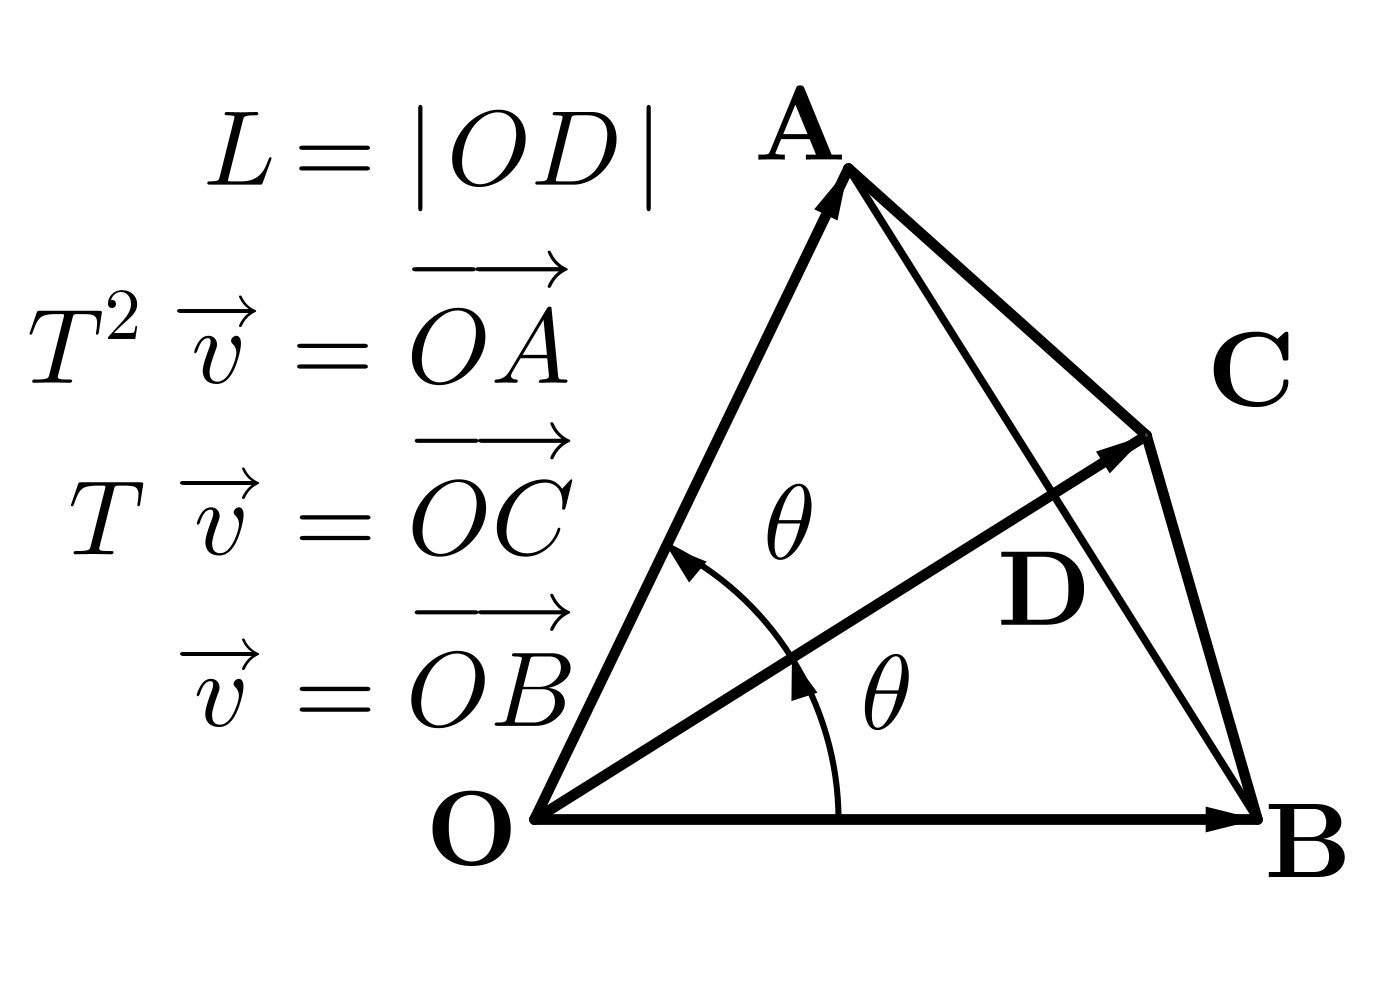
\includegraphics[width=4.4cm,height=3.2cm,scale=0.22]{diagram5BI-1.png}\Blind{\quad}\vspace{-76pt}\parSol{}
Othws, let $\Span{v,Tv}=\Rbb^2.$ Let $L=x^2+y^2,$ where $v=\Par{x,y}.$\parSol{}
Supp $p\Par{z}=z^2+bz+c.$ Let $P=L\cos\theta\Rightarrow L\big/2P=1\big/\Par{2\cos\theta}.$\parSol{}
Then $Tv=\BigPar{L\big/2P}\Par{T^2 v+v}\Rightarrow T=\BigPar{L\big/2P}\Par{T^2+I}.$\parSol{}
Hence $p\Par{T}=T^2-2\cos\theta\, T+I=0.$\PfEnd\vspace{4pt}\parSol{}
\Or Let $\Par{e_1,e_2}$ be the std bss of $\Rbb^2.$ Becs $Te_1=\cos\theta\;e_1+\sin\theta\;e_2,\;T^2e_1=\cos2\theta\;e_1+\sin2\theta\;e_2.$\vspace{0pt}\parSol{}
$ce_1+bTe_1=-T^2 e_1\Longleftrightarrow{}${\small$\begin{pmatrix}1 & \cos\theta\\0 & \sin\theta\end{pmatrix}\begin{pmatrix}c \\ b\end{pmatrix}$}${}={}${\small$\begin{pmatrix}-\cos2\theta\\-\sin2\theta\end{pmatrix}$}. Now $\det=\sin\theta\neq 0,c=1,b=2\cos\theta.$\PfEnd%\vspace{10pt}\parSol{}
%\Or $\Mt[\BigPar]{T,\Par{e_1,e_2}}={}${\small$\begin{pmatrix}\Blind{-}\cos\theta & \sin\theta\\-\sin\theta & \cos\theta
%\end{pmatrix}$}. By (4E 11), $\Par{z\pm 1}$ or $\Par{z^2-2\cos\theta\,z+1}$ is the min.\PfEnd
\SepLine

%\Anchor{5BI4e9}\ProblemBnoor{{4E 9}}{
%	\TextA{Supp $T\in\Lm{V}$ with the min $p=c_0+c_1z+\dots+c_{m-1}z^{m-1}+z^m,$}
%	\TextA{and $A=\Mt{T,B_V}$ is suth each $A_{j,k}\in\Qbb.$ Explain why all $c_k\in\Qbb.$}
%}Let $b_0I+b_1A+\dots+b_{m-1}A^{m-1}=-A^m.$ \,A system of $n^2$ liney equations in $m$ unknowns.\parSol{}
%Becs each $\Par{A^i}{_{j,k}}\in\Qbb\Rightarrow b_i\in\Qbb.$ 又 $\Par{c_0,\dots,c_{m-1}}$ is a solus.\PfEnd
%\SepLine

\Anchor{5BI4e11}\ProblemBnoor{4E 11}{
	\TextA{Supp $V$ is 2\hspace{1pt}-\hspace{1pt}dim, $T\in\Lm{V}$ with the min $p$, and $\Mt[\BigPar]{T,\Par{v,w}}={}${\large$\begin{pmatrix} a &\hspace{-4pt} c\\[-4pt] b &\hspace{-4pt} d\end{pmatrix}.$}\vspace{-8pt}}
	\PrePa\TextA{Show $q\Par{z}=z^2-\Par{a+d}z+\Par{ad-bc}$ is a multi of $p.$}
	\PrePb\TextA{Show if $b=c=0$ and $a=d,$ then $p\Par{z}=z-a;$\;othws $p=q.$}
}(a) $Tv=av+bw\Rightarrow\Par{T-aI}v=bw\Rightarrow\Par{T-dI}\Par{T-aI}v=bTw-bdw=bcv.$\parSol{\Ha}
$Tw=cv+dw\Rightarrow \Par{T-dI}w=cv\Rightarrow\Par{T-aI}\Par{T-dI}w=cTv-acv=bcw.$\vspace{2pt}\parSol{}
(b) {\vspace{-2pt}\FontSmall If $b=c=0$ and $a=d.$ Then $\Mt{T}=a\Mt{I}\Rightarrow T=aI.$ Othws, we show $T\not\in\Span{I},$}\parSol{\Hb}
{\vspace{-2pt}\FontSmall so that $\deg p=\dim V.$ Let (1) $a=d,$ (2) $b=0,$ (3) $c=0.$ Then (1), (2) and (3) cannot be all true.}\parSol{\Hb}
{\vspace{-2pt}\FontSmall(I) Asum (1) is true, with (2) or (3) not true. Then $Tv=av+bw,$ or $Tw=cv+aw\not\in\Span{w}.$}\parSol{\Hb}
{\vspace{-2pt}\FontSmall(II) Asum (2) or (3) are true, with (1) not true. Then $Tv=av+bw,$ or $Tw=cv+dw.$}\PfEnd
\SepLine

\Anchor{5BI4e17}\ProblemBnoor{{4E 17}}{
	\TextA{Supp $V$ finide, $T\in \Lm{V}$ with the min $p,$ and $\lambda\in\Fbb.$}
	\TextA{Show the min $s$ of $\Par{T-\lambda I}$ is $q\Par{z}=p\Par{z+\lambda}.$}
}Becs $q\Par{T-\lambda I}=p\Par{T}=0\Rightarrow q$ a multi of $s\Rightarrow\deg q=\deg p\geqslant\deg s.$\parSol{}
Define $r\Par{z}=s\Par{z-\lambda}\Rightarrow r\Par{T}=s\Par{T-\lambda I}=0\Rightarrow \deg r=\deg s\geqslant\deg p.$\PfEnd\vspace{2pt}\parSol{}
\Or Becs  $T^k\in\Span{I,T,\dots,T^{k-1}}\Longleftrightarrow\Par{T-\lambda}{^k}\in\Span[\BigBigPar]{I,\Par{T-\lambda I},\dots,\Par{T-\lambda I}{^{k-1}}}.$\PfEnd
\SepLine

\Anchor{5BI4e18}\ProblemBnoor{{4E 18}}{
	\TextA{Supp $V$ is finide, $T\in\Lm{V}$ with the min $p$ of deg $m,$ and $\lambda\neq 0.$}
	\TextA{Show the min $s$ of $\lambda T$ is $q\Par{z}=\lambda^m p\BigPar{{z}\big/{\lambda}}.$}
}Becs $q\Par{\lambda T}=\lambda^m p\Par{T}=0\Rightarrow q$ is multi $s\Rightarrow\deg q=\deg p\geqslant\deg s.$\parSol{}
Define $r\Par{z}=s\Par{\lambda z}\Rightarrow r\Par{T}=s\Par{\lambda T}=0\Rightarrow \deg r=\deg s\geqslant\deg p.$\PfEnd\vspace{2pt}\parSol{}
\Or Becs $\Par{\lambda T}{^k}\in\Span[\BigBigPar]{\lambda I,\lambda T,\dots,\Par{\lambda T}{^{k-1}}}\Longleftrightarrow T^k\in\Span{I,T\dots,T^{k-1}}.$\PfEnd
\SepLine

%\Anchor{5BI4e16}\ProblemBnoor{4E 16}{
%	\TextB{Supp $a_0 ,\dots, a_{n-1}\in\Fbb.$ Let $T$ be the optor on $\Fbb^n$ suth\vspace{2pt}}
%	\TextB{$\Mt{T}={}${\normalsize$\begin{pmatrix}
%	0 &\hspace{-4pt}   &\hspace{-4pt} &\hspace{-4pt} &\hspace{-4pt} & -a_0\\[-4pt]
%	1 &\hspace{-4pt} 0 &\hspace{-4pt} &\hspace{-4pt} &\hspace{-4pt} & -a_1\\[-4pt]
%	  &\hspace{-4pt} 1 &\hspace{-4pt} \ddots &\hspace{-4pt} &\hspace{-4pt} & \vdots\\[-4pt]
%	  &\hspace{-4pt}   &\hspace{-4pt} \ddots &\hspace{-4pt} &\hspace{-4pt} 0 & -a_{n-2} \\[-4pt]
%	0 &\hspace{-4pt}   &\hspace{-4pt} &\hspace{-4pt}  &\hspace{-4pt} 1 & -a_{n-1}
%\end{pmatrix} $}, wrto the std bss $\Par{e_1,\dots,e_n}$.\vspace{4pt}}
%	\TextB{Show the min poly of $T$ is $\,p\,$ defined by $p\Par{z}=a_0 + a_1 z + \dots + a_{n-1} z^{n-1} + z^n$.}
%}Note that $\Par{e_1,Te_1,\dots,T^{n-1}e_1}$ is liney indep. 又 The deg of min poly is at most $n.$\par\quad
%$T^n e_1=\cdots=T^{n-k}e_{1+k}=\cdots=T e_n=-a_0 e_1-a_1 e_2-a_2 e_3-\dots-a_{n-1}e_n$\par
%$=\Par{-a_0 I-a_1 T-a_2 T^2-\dots-a_{n-1}T^{n-1}}e_1.$ Thus $p\Par{T}e_1=0=p\Par{T}e_j$ for each $e_j=T^{j-1}e_1.$\PfEnd
%\SepLine

%\BulletPointX{\Large\textsc{Eigenvalues On Odd-Dimensional Real Vector Spaces}}\par
%\ProblemB{
%	\textsc{Even-Dimensional Null Space}\TextB{}
%	\TextB{Supp $\Fbb=\Rbb,$ $V$ is finide, $T\in\Lm{V}$ and $b, c\in\Rbb$ with $b^2 < 4c$.}
%	\TextB{Prove $\dim\Null\Par{T^2 + bT + cI}$ is an even number.}
%}\par\quad
%Denote $\Null\Par{T^2 + bT + cI}$ by $R.$ Then $T\mmid_R+bT\mmid_R+cI_R=\Par{T+bT+cI}\mmid_R=0\in\Lm{R}.$\par\quad
%Supp $\lambda$ is an eigval of $T_R$ with an eigvec $v\in R.$\par\quad
%Then $0=\Par{T\mmid_R^2+bT\mmid_R+cI_R}\Par{v}=\Par{\lambda^2+\lambda b+c}v=\BigPar{\Par{\lambda+b}^2+c-\Frac{b^2}{4}}v.$\par\quad
%Becs $c-\Frac{b^2}{4}>0$ and we have $v=0.$ Thus $T_R$ has no eigvals.\par\quad
%Let $U$ be invarsp of $R$ that has the largest, even dim among all invarsps.\par\quad
%Asum $U\neq R.$ Then $\exists\,w\in R$ but $w\not\in U.$ Let $W$ be suth $\Par{w,T\mmid_R w}$ is a bss of $W.$\par\quad
%Becs $T\mmid_R^2 w=-bT\mmid_R w-cw\in W.$ Hence $W$ is invarsp of dim $2.$\par\quad
%Thus $\dim \Par{U+W}=\dim U+2-\Dim\Par{U\cap W},$ where $U\cap W=\zeroSubs,$\par\qquad\qquad
%for if not, becs $w\not\in U,T\mmid_R w\in U,$\par\qquad\qquad $U\cap W$ is invard $T\mmid_R$ of one dim ( impossible becs $T\mmid_R$ has no eigvecs ).\par\quad
%Hence $U+W$ is even-dim invarsp under $T\mmid_R$, ctradic the max of $\dim U.$\par\quad
%Thus the asum was incorrect. Hence $R=\Null\Par{T^2+bT+cI}=U$ has even dim.\PfEnd
%\SepLine
%
%\ProblemB{
%	\textsc{Operators On Odd-Dimensional Vector Spaces Have Eigenvalues}\TextB{}
%	\PrePa\TextB{Supp $\Fbb=\Cbb.$ \tgnr\large Then by [5.21], done.}
%	\PrePb\TextB{Supp $\Fbb=\Rbb,$ $V$ is finide, and $\dim V=n$ is an odd number.}
%	\Blind{\PrePb}\TextB{Let $T\in\Lm{V}$ and the min poly is $\,p\,$. Prove $T$ has an eigval.}
%}\par\quad
%(i) If $n=1,$ then done.\par\quad\Endi
%(ii) Supp $n\geqslant 3.$ Asum every optor, on odd-dim vecsps of dim less than $n,$ has an eigval.\par\quad\Hii
%If $p$ is a poly multi of $\Par{x - \lambda}$ for some $\lambda\in\Rbb,$ then by [8.49] $\lambda$ is an eigval of $T$ and done.\par\quad\Hii
%Now supp $b, c\in\Rbb$ suth $b^2 < 4c$ and $p$ is a poly multi of $x^2 + bx + c$ (see [4.17]).\par\quad\Hii
%Then $\exists\,q\in\PoRi$ suth $p\Par{x} = q\Par{x}\Par{x^2 + bx + c}$ for all $x\in\Rbb.$\par\quad\Hii
%Now $0 = p\Par{T} = \BigPar{q\Par{T}}\Par{T^2 + bT + cI},$ which means that $q\Par{T}\mmid_{\Range\Par{T^2+bT+cI}}=0.$\par\quad\Hii
%Becs $\deg q < \deg p$ and $p$ is the min poly of $T$, hence $\Range\Par{T^2 + bT + cI}\neq V$.\par\quad\Hii
%又 $\dim V$ is odd and $\dim\Null\Par{T^2 +bT+cI}$ is even ( by our previous result ).\par\quad\Hii
%Thus $\dim V - \dim \Null\Par{T^2 + bT + cI}=\dim \Range\Par{T^2 + bT + cI}$ is odd.\par\quad\Hii
%By [5.18], $\Range\Par{T^2 + bT + cI}$ is invarsp of $V$ under $T$ that has odd dim less than $n.$\par\quad\Hii
%Our induc hypo now implies that $T\mmid_{\Range\Par{T^2 + bT + cI}}$ has an eigval.\par\quad
%By induc.\PfEnd
%\SepLine

%\Anchor{5BI2e24}\ProblemBnoor{{2E 24}}{
%	\TextB{Supp $\Fbb=\Rbb,T\in\Lm{V}$ has no eigvals. Prove every invarsp $U$ is even-dim.}
%}Asum $\dim U$ is odd. Then $\exists$ eigval of $T\mmid_U,$ so of $T\Rightarrow\exists$ $1$\hspace{1pt}-\hspace{1pt}dim invarsp, ctradic.\PfEnd
%\SepLine

\Anchor{5BI4e29}\ProblemBnoor{{4E 29}}{
	\TextB{Supp $V$ is finide, $\dim V=n\geqslant 2$, and $T\in\Lm{V}.$ Show $T$ has a $2$\hspace{1pt}-\hspace{1pt}dim invarsp.}
}See [9.8] for a graceful proof. \Or Let each $V_{\!k}$ be an arb vecsp of dim $k$ with an arb $T_{\!k}\in\Lm{V_{\!k}}.$\par\quad
Define the stmt $P\Par{k}:$ every optor on a $V_{\!k}$ has invarsp of dim $2.$ (i) $k=2.$ Immed.\par\quad
(ii) $k\geqslant 2.$ Asum $P\Par{k}$ holds. Let $p$ be the min of $T_{\!k+1}=T.$ Note that $V_{\!k+1}$ non0 $\Rightarrow p$ nonC, $\deg p\geqslant 1.$\par\quad
(a) If $p\Par{z}=\Par{z-\lambda}q\Par{z},$ then by (4E 5.A.39), $\exists\,U$ invarspd $T$ of dim $k.$\par\quad\Ha
By asum, the optor $T\mmid_U$ on a $k$\hspace{1pt}-\hspace{1pt}dim vecsp has invarsp of dim $2$, so has $T.$\vspace{2pt}\par\quad
(b) Othws, $T_{\!k+1}$ has no eigvals $\Rightarrow p$ of deg $\geqslant 1$ has no zeros, thus $\Fbb=\Rbb,$ and $\deg p$ is even.\par\quad\Hb
Let $p\Par{z}=\Par{z^2+b_1z+c_1}\cdots\Par{z^2+b_mz+c_m}\Rightarrow\exists\,\Par{T^2+b_jT+c_j}$ not inje\par\quad\Hb
$\Rightarrow\exists\,v\neq 0,\Par{T^2+b_jT+c_j}v=0\Rightarrow T^2v\in\Span{v,Tv},$ invard $T,$ while $\dim\Span{v,Tv}=2.$\PfEnd
\SepLine

\Anchor{5BIN5.32}\ProblemBnoor{4E 5.32}[\Sbra]{
	\TextB{Supp $T\in\Lm{V}$ with the min $p.$ Prove $T$ not inje $\Longleftrightarrow$ the const term of $p$ is $0.$}
	}$T$ not inje $\Longleftrightarrow 0$ is eigval of $T$ $\Longleftrightarrow 0$ is zero of $p \Longleftrightarrow 0$ the const term of $p.$\PfEnd\vspace{2pt}\parSol{}
\Or Supp $p\Par{0}=\Par{z-0}\Par{z-\lambda_1}\cdots\Par{z-\lambda_m}=0\Rightarrow T\Par{T-\lambda_1 I}\cdots\Par{T-\lambda_m I}=0.$\parSol{}
又 $p$ is the min $\Rightarrow q\Par{T}=\Par{T-\lambda_1}\cdots\Par{T-\lambda_m}\neq 0.$ \,Now $0=p\Par{T}=Tq\Par{T}\Rightarrow T$ not inje.\PfEnd
\SepLine

\ChEnd

\pagebreak

\ChDecl{Ch5BII}{5.B: II}{\qquad{\small\textbf{注意\,:}\;这一节的题号主要使用第四版5.C节}}%\orMode{\hLk{5BII9}{9}\;\;\hLk{5BII14}{14}\;\;\hLk{5BII15}{15}\;\;\hLk{5BII20}{20}\;\;|\;\;\hLk{5BII4e1}{4E: 1,}\;\;\hLk{5BII4e2}{2,}\;\;\hLk{5BII4e3}{3,}\;\;\hLk{5BII4e4}{4,}\;\;\hLk{5BII4e5}{5,}\;\;\hLk{5BII4e6}{6,}\;\;\hLk{5BII4e7}{7,}\;\;\hLk{5BII4e8}{8,}\;\;\hLk{5BII4e9}{9,}\;\;\hLk{5BII4e10}{10}\;\;\hLk{5BII4e11}{11,}\;\;\hLk{5BII4e12}{12,}\;\;\hLk{5BII4e13}{13,}\;\;\hLk{5BII4e14}{14}}{[1]: ; [2]: ; [3]: .}

\vspace{4pt}

\Anchor{5BII4e2}\ProblemN{2}{
	\TextA{Supp $A$ and $B$ are up-trig \Par{and square} matrices of the same size,}
	\TextA{with $\alpha_1 , \dots , \alpha_n$ on the diag of $A$ and $\beta_1 , \dots , \beta_n$ on the diag of $B$.}
	\PrePa\TextA{Show $A + B$ up-trig with $\alpha_1 + \beta_1 , \dots , \alpha_n + \beta_n$ on the diag.}
	\PrePb\TextA{Show $AB$ up-trig with $\alpha_1 \beta_1 , \dots , \alpha_n \beta_n$ on the diag.}
}(a) By def, immed. \:(b) Becs $A_{j,k}=B_{j,k}=0$ for $j>k.$ By def, for each $p\in\Bra{1,\dots,n},$\parSol{} $\Par{AB}{_{p,p}}=A_{p,1}B_{1,p}+\dots+A_{p,p-1}B_{p-1,p}+A_{p,p}B_{p,p}+A_{p,p+1}B_{p+1,p}+\dots+A_{p,n}B_{n,p}=A_{p,p}B_{p,p}.$\PfEnd
\SepLine

\Anchor{5BII4e3}\ProblemN{3}{
	\TextA{Supp $T$ inv, $B_V=\Par{v_1,\dots,v_n},$ $\Mt{T}=A$ is up-trig,}
	\TextA{with $\lambda_1,\dots,\lambda_n$ on diag. Show $A^{-1}$ is also up-trig, with $\lambda_1^{-1},\dots,\lambda_n^{-1}$ on diag.}
}Becs $\lambda_k$ on diag of $A$ $\Longleftrightarrow\lambda_k$ eigval of $T$ $\Longleftrightarrow\lambda_k^{-1}$ eigval of $T^{-1}$ $\Longleftrightarrow\lambda_k^{-1}$ on diag of $A^{-1}.$\PfEnd\vspace{2pt}\par\quad
\Or Let each $Tv_k=u_k+\lambda_kv_k,$ where $u_k\in\Span{v_1,\dots,v_{k-1}}.$ We use induc on $k.$\par\quad
(i) $k=1.$ $Tv_1=\lambda_1v_1\Rightarrow T^{-1}v_1=\lambda_1^{-1}v_1\in\Span{v_1},$ invard $T^{-1};$ and $\lambda_1^{-1}$ is the 1st ent on diag.\par\quad\Endi
(ii) $k\geqslant 2.$ Asum $\Span{v_1,\dots,v_{k-1}}$ invard $T^{-1}.$\par\quad\Hii
Note that $Tv_k=u_k+\lambda_kv_k\Rightarrow v_k=T^{-1}\Par{c_1v_1+\dots+c_{k-1}v_{k-1}}+\lambda_kT^{-1}v_k.$\par\quad\Hii
Thus $T^{-1}v_k=\lambda_k^{-1}v_k-\lambda_k^{-1}T^{-1}u_k\in\Span{v_1,\dots,v_k},$ invard $T;$ and $\lambda_{k}^{-1}$ is the $k^\text{th}$ ent on diag.\PfEnd
\SepLine

%\Anchor{5BII14}\Anchor{5BII4e4}\ProblemNor{4}{3E 5.B.14}{
%	\TextA{Give an inv $T$ and a $B_V$ suth each $\Mt{T}{_{k,k}}=0.$}
%}Define $T\in\Lm{\Rbb^2}:\Par{x,y}\mapsto\Par{y,x}.$
%\SepLine
%
%\Anchor{5BII15}\Anchor{5BII4e5}\ProblemNor{5}{3E 5.B.15}{
%	\TextA{Give a non-inv $T$ and a $B_V$ suth each $\Mt{T}{_{k,k}}\neq 0.$}
%}Define $T\in\Lm{\Fbb^2}:\Par{z,w}\mapsto\Par{z+w,z+w}.$
%\SepLine

%\Anchor{5BII20}\Anchor{5BII4e6}\ProblemNor[]{6}{3E 5.B.20}{
%	\TextA{Supp $\Fbb=\Cbb,$ $V$ is finide, $T\in\Lm{V},$ and $k\in\Bra{1,\dots,\dim V}.$}
%	\TextA{Prove $V$ has a $k$\hspace{1pt}-\hspace{1pt}dim invarspd $T.$\hfill\FontNorm\tgnr By [5.27] and [5.26], immed.\vspace{-3pt}}
%}\SepLine

\Anchor{5BII4e8}\ProblemN{8}{
	\TextA{Supp $V$ is finide, and $v\in V$ is non0 suth $q\Par{T}v=0,$ where $q\Par{z}=z^2+2z+2.$}
	\PrePa\TextA{Supp $\Fbb=\Rbb.$ Prove $\nexists\,B_V$ suth $\Mt{T}$ up-trig.}
	\PrePb\TextA{Supp $\Fbb=\Cbb,$ and $\exists\,B_V$ suth $A=\Mt{T}$ up-trig. Prove $-1+\i$ or $-1-\i$ on the diag.}
}Define $p_v$ as (4E 3.C.7). Note that $\deg p_v\geqslant 1$ becs $v\neq 0.$ 又 $q\Par{T\mmid_{\nullp p_v\SmallPar{v}}}=0.$\parSol{}
Now $q$ of deg $2$ is a multi of the min of $T\mmid_{\nullp p_v\SmallPar{v}},$ which is $p_v,$ of which the min of $T$ is a multi.\parSol{}
(a) Note that $q$ has no $1$\hspace{1pt}-\hspace{1pt}deg factors $\Rightarrow\deg p_v\geqslant 2.$ By [4E 5.44].\parSol{}
(b) $q\Par{z}=\Par{z+1+\i}\Par{z+1-\i}\Rightarrow -1-\i$ or $-1+\i$ zero of $p_v\Rightarrow$ is eigval $\Rightarrow$ on diag.\PfEnd
\SepLine

\Anchor{5BII4e9}\ProblemN{9}{
	\TextA{Supp $B\in\Cbb^{n,n}.$ Prove $\exists$ inv $A\in\Cbb^{n,n}$ suth $A^{-1} BA$ is up-trig.}
}Define $T\in\Cbb^n$ with $B=\Mt[\BigPar]{T,\Par{e_1,\dots,e_n}}.$ Let $C=\Mt[\BigPar]{T,\Par{f_1,\dots,f_n}}$ be up-trig.\parSol{}
Let $A=\Mt[\BigPar]{I,\,f\rightarrow e}.$ Then $C=A^{-1}BA.$\PfEnd
\SepLine

\Anchor{5BII4e10}\ProblemN{10}{
	\TextA{Supp $B_V=\Par{v_1,\dots,v_n},A=\Mt{T,B_V}.$ Show the following are equiv\hspace{1pt}$:$}
	\PrePa\TextA{$A$ is low-trig. \:{\tgnr\large(b)} Each $Tv_k\in\Span{v_k,\dots,v_n}.$ \:{\tgnr\large(c)} Each $\Span{v_k,\dots,v_n}$ invard $T.$}
}By def, (a) and (b) are equiv, and (c) $\Rightarrow$ (b). Now supp (b) holds. For any $k\in\Bra{1,\dots,n}.$\parSol{}
$Tv_k\in\Span{v_k,\dots,v_n},\,Tv_{k+1}\in\Span{v_{k+1},\dots,v_n},\cdots,\,Tv_{n}\in\Span{v_n}.$ Thus (c) holds.\PfEnd
\SepLine

\BulletPointX\TipsN{1}\;\;Supp $B_V=\Par{v_1,\dots,v_n},B_{V\apostrophe}=\Par{\varphi_1,\dots,\varphi_n},T\in\Lm{V},A=\Mt{T,B_V}.$\TextB{}
\IndentTipsN{1}(a) $A$ up-trig $\Longleftrightarrow T=\sum_{k=1}^n\sum_{j=1}^kA_{j,k}E_{k,j}\Longleftrightarrow T\apostrophe=\sum_{k=1}^n\sum_{j=1}^kA^t_{k,j}\reflectbox{\textit{E}}{_{j,k}}\Longleftrightarrow A^t$ low-trig.\TextB{}
\IndentTipsN{1}(b) $A$ low-trig $\Longleftrightarrow T=\sum_{k=1}^n\sum_{j=1}^kA_{k,j}E_{j,k}\Longleftrightarrow T\apostrophe=\sum_{k=1}^n\sum_{j=1}^kA^t_{j,k}\reflectbox{\textit{E}}{_{k,j}}\Longleftrightarrow A^t$ up-trig.
\SepLine

\Anchor{5BII4e11}\ProblemBX{\TipsN{2}}{
	\TextA{Supp $\Par{\alpha_1,\dots,\alpha_n},\Par{\beta_1,\dots,\beta_n}$ are bses of $V,$ with each $\alpha_k=\beta_{n-k+1}.$}
	\TextA{Prove $\Mt{T,\alpha\rightarrow\alpha}$ up-trig $\Longleftrightarrow\Mt{T,\beta\rightarrow\beta}$ low-trig.}
}For each $k\in\Bra{1,\dots,n},\:T\beta_{n-k+1}=T\alpha_k\in\Span{\alpha_1,\dots,\alpha_k}=\Span{\beta_n,\dots,\beta_{n-k+1}}.$\PfEnd
\SepLine

\pagebreak

\Anchor{5BII4e12}\ProblemN{12}{
	\TextA{Supp $V$ is finide, $U$ invarspd $T,$ and $\Mt{T}$ is up-trig for some $B_V.$}
	\PrePa\TextA{Prove $\Mt{T\mmid_U}$ up-trig for some $B_U$. \, {\tgnr\large(b)} Prove $\Mt{T\XSlash U}$ up-trig for some $B_{V\XSlash U}.$}
}Becs the min $\Par{z-\lambda_1}\cdots\Par{z-\lambda_m}$of $T$ is multi of min of $T\mmid_U$ and of min of $T\XSlash U.$\PfEnd
\SepLine

\Anchor{5BII4e13}\ProblemN{13}{
	\TextA{Supp $V$ is finide, $U$ invarspd $T$ suth $T\mmid_U,T\XSlash U$ up-trig. Prove $T$ up-trig.}
}Let $B_U=\Par{u_1,\dots,u_p},B_{V\XSlash U}=\Par{w_1+U,\dots,w_q+U}$ suth $\Mt{T\mmid_U},\Mt{T\XSlash U}$ up-trig.\parSol{}
Then each $Tu_k\in\Span{u_1,\dots,u_k}$ and each $Tw_j+U\in\Span{w_1+U,\dots,w_j+U}.$\parSol{}
By (3.E.13), $B_V=\Par{u_1,\dots,u_p,w_1,\dots,w_q}.$ Now each $Tw_j\in\Span{u_1,\dots,u_p,w_1,\dots,w_j}.$\PfEnd
\SepLine

\Anchor{5BII4e14}\ProblemN{14}{
	\TextA{Supp $V$ is finide. Prove $T$ up-trig $\Longleftrightarrow$ $T\apostrophe$ up-trig.}
}Immed, by \TIPSN{1} and \TIPSN{2}, \OR by (4E 18) and [4E 5.44].\PfEnd
\SepLine
\ChEnd

\ChDecl{Ch5C}{5.C \& [4E] 5.D}{}

\vspace{4pt}


\Anchor{5C1}\ProblemN{1}{
	\TextA{Supp $T\in\Lm{V}$ is diag. Prove $V=\null T\oplus\range T.$}
}Let $\lambda_1,\dots,\lambda_m$ be the dist non0 eigvals of $T.$ Then $\range T=E\Par{\lambda_1,T}\oplus\cdots\oplus E\Par{\lambda_m,T}.$\parSol{}
Becs $\null T=E\Par{0,T}.$ If $0$ is eigval, then done. Othws, $E\Par{0,T}=\zeroSubs$ and done.\PfEnd
\PfEnd
\Anchor{5C2}\AExa Convly not true. Define the inv $T\in\Lm{\Rbb^2}:\Par{x,y}\mapsto\Par{{-y,x}}.$ No eigvals.
\SepLine

\Anchor{5C1'}\ProblemB{
	\TextB{Supp $T\in\Lm{V},V=\null T\oplus\range T,$ $U$ invarspd $T.$ Show $U=\null T\mmid_U\oplus\range T\mmid_U.$}
}Becs $\null T\mmid_U\cap\range T\mmid_U\subseteq\null T\cap\range T=\zeroSubs.$ By Exe (3).\PfEnd
\SepLine

\Anchor{5C5}\ProblemN{5}{
	\TextA{Supp $\Fbb=\Cbb,$ $V$ is finide, and $T\in\Lm{V}$ with dist eigvals $\lambda_1,\dots,\lambda_m.$}
	\TextA{Supp $V=\null S_j\oplus\range S_j$ for each $S_j=T-\lambda_jI.$ Prove $T$ is diag.}
}
\SepLine

\Anchor{5C7}\ProblemN{7}{
	\TextA{Supp $T\in\Lm{V},A=\Mt{T,B_V}$ is diag. Prove $A$ has $\dim E\Par{\lambda,T}$ $\lambda$'s on diag.}
}Given $B_V=\Par{v_1,\dots,v_n}.$ Becs $T$ diag. Each $Tv_k=\lambda_jv_k.$ Forming $B_{E\SmallPar{\lambda_j,T}}.$ Immed.\PfEnd
\SepLine

\Anchor{5C4e13}\ProblemBnoor{4E 13}{
	\TextA{Supp $A,B\in\Fbb^{n,n}$ and $A$ is diag with {\tgsc dist} ents on diag. Prove $AB=BA\Longleftrightarrow B$ is diag.}
}\NOTICE that for any diag $C,$ each $C_{j,k}=0$ for $j\neq k.$\parSol{}
Becs (I) $A_{j,j}B_{j,k}=A_{j,1}B_{1,k}+\dots+\Sbra{A_{j,j}B_{j,k}}+\dots+A_{j,n}B_{n,k}=\Par{AB}{_{j,k}}.$\parSol{}
And (II) $B_{j,k}A_{k,k}=B_{j,1}A_{1,k}+\dots+\Sbra{B_{j,k}A_{k,k}}+\dots+B_{j,n}A_{n,k}=\Par{BA}{_{j,k}}.$\parSol{}
Supp $B$ diag. If $j=k,$ then $\Par{BA}{_{j,k}}=\Par{AB}{_{j,k}},$ othws true as well.\parSol{}
Supp $AB=BA\Rightarrow A_{j,j}B_{j,k}=A_{k,k}B_{j,k}.$ Asum $B_{j,k}\neq0$ with $j\neq k.$ Then $A_{j,j}=A_{k,k},$ ctradic.\PfEnd
\SepLine\pagebreak

\Anchor{5C4e14}\ProblemBnoor{4E 14}{
	\TextA{Supp $\Fbb=\Cbb,$ $k\in\Nbp,$ and $T\in\Lm{V}$ is inv. Prove $T^k$ diag $\Rightarrow T$ diag.}
}%Using Exe (4E 13). Supp $\Mt{T^k,B_V}=A$ diag. Let $B=\Mt{T^{-1},B_V},C=\Mt{T,B_V}.$\parSol{}
%Now $T^kT^{-1}=T^{-1}T^k\Rightarrow AB=BA\Rightarrow T^{-1}$ diag. Then $T^{-1}T=TT^{-1}\Rightarrow BC=CB\Rightarrow T$ diag.\PfEnd
\AExa Not true if $\Fbb=\Rbb.$ Define $T\in\Lm{\Rbb^2}:\Par{x,y}\mapsto\Par{{-y,x}}.$ No eigvals.
\SepLine

\Anchor{5C4e15}\ProblemBnoor{4E 15}{
	\TextB{Supp $\Fbb=\Cbb,$ $V$ is finide, $T\in\Lm{V}$ with the min $p.$ Prove the following equiv\hspace{1pt}$:$}
	\PrePa\TextB{$T$ diag. \, {\tgnr\large(b)} $\nexists\,\lambda\in\Cbb$ suth $p$ is multi of $\Par{z-\lambda}{^2}.$}
	\PrePc\TextB{$p$ and $p\apostrophe$ have no common zeros. \, {\tgnr\large(d)} $\gcd\Par{p,p\apostrophe}=1.$}
}\SepLine

\Anchor{5C4e17}\ProblemBnoor{4E 17}{
	\TextA{Supp $V$ is finide. Prove $\Lm{V}$ has a bss consisting of diag optors.}
}Let $B_V=\Par{v_1,\dots,v_n}.$ Define each $E_{j,k}\in\Lm{V}:v_x\mapsto\delta_{j,x}v_k\Rightarrow$ [5.41](c) true.\PfEnd
\SepLine

\Anchor{5C4e18}\ProblemBnoor{4E 18}{
	\TextA{Supp $T\in\Lm{V}$ is diag. Prove if $U$ invarspd $T,$ then $T\XSlash U\in\Lm{V\XSlash U}$ is diag.}
}Supp the eigvecs of $T$ are $B_V=\Par{v_1,\dots,v_n}$ with corres eigvals $\lambda_1,\dots,\lambda_n.$\parSol{}
By \Sbra{5.A \TIPSN{3}}, $B_U=\Par{v_{k_1},\dots,v_{k_m}}.$ Let $\Par{v_1,\dots,v_n}=\Par{v_{k_1},\dots,v_{k_m},\dots,v_{k_n}}.$\parSol{}
Let $B_{V\XSlash U}=\Par{v_{k_{m+1}}+U,\dots,v_{k_n}+U}.$ Becs each $\BigPar{T\XSlash U}\Par{v_{k_{m+j}}+U}=\lambda_{k_{m+j}}\Par{v_{k_{m+j}}+U}.$\PfEnd\vspace{3pt}\parSol{}
\Or Becs the min of $T$ is multi of that of $T\XSlash U.$ By [4E 5.62].\PfEnd
\SepLine

\Anchor{5C4e19}\ProblemBnoor{4E 19}{
	\TextA{Give an exa of $T\in\Lm{V}$ not diag while $T\mmid_U,T\XSlash U$ both diag, where $U$ invarspd $T.$}
}Define $T\in\Lm{\Rbb^3}:\Par{x,y,z}\mapsto\Par{z,x,y}.$ Then $1$ is the only eigval with $\dim E\Par{1,T}=1.$\PfEnd
\SepLine

\Anchor{5C4e20}\ProblemBnoor{4E 20}{
	\TextA{Supp $V$ is finide, $T\in\Lm{V}.$ Prove $T$ diag $\Longleftrightarrow T\apostrophe$ diag.}
}By (4E 5.B.28), $T,T\apostrophe$ have the same min poly. By [4E 5.62].\PfEnd\vspace{2pt}\parSol{}
\Or By \Sbra{5.B(II) \TIPSN{1}}. Note that low-trig and up-trig $\Longleftrightarrow$ diag.\PfEnd
\SepLine

\Anchor{5C16}\ProblemN{16}{
	\TextA{Define $F_1=1,F_2=2,$ and $F_n=F_{n-1}+F_{n-2}$ \:for $n\geqslant 3.$\vspace{6pt}}
	\TextA{Define $T\in\Lm{\Rbb^2}:\Par{x,y}\mapsto\Par{y,x+y}.$ \, (a) Find all eigvals and eigvecs of $T.$\vspace{-6pt}}
	\PrePb\TextA{Show each $T^n\Par{0,1}=\Par{F_n,F_{n+1}},$ \, (c) and each $F_n={}${\LARGE$\frac{1}{\sqrt{5}\;}$}$\,\bigg[\bigg(\!${\LARGE$\frac{\:1\,+\,\sqrt{5}\:}{2}$}$\!\bigg)\begin{array}{l}\hspace{-5pt}{}_n\\\\\vspace{-18pt}\end{array}\hspace{-8pt}-\bigg(\!${\LARGE$\frac{\:1\,-\,\sqrt{5}\:}{2}$}$\!\bigg)\begin{array}{l}\hspace{-5pt}{}_n\\\\\vspace{-18pt}\end{array}\hspace{-5pt}\bigg].$\vspace{-4pt}}
%	\PrePd\TextA{Show each $F_n$ is the integer that closest to {\LARGE$\frac{1}{\sqrt{5}\;}$}$\,\bigg(\!${\LARGE$\frac{\:1\,+\,\sqrt{5}\:}{2}$}$\!\bigg)\begin{array}{l}\hspace{-5pt}{}_n\\\\\vspace{-18pt}\end{array}\hspace{-8pt}.$\vspace{-8pt}}
}(a) Supp $\lambda\Par{x,y}=\Par{y,x+y}$ with $x$ or $y$ non0. Note that $x=0\Longleftrightarrow y=0,$ and $0$ is not eigval.\parSol{\Ha}
Then $\lambda_1={}${\Large$\frac{\:1\,+\,\sqrt{5}\:}{2}$}, $v_1=\Par{1,\frac{1+\sqrt{5}}{2}};$
\,and $\lambda_2={}${\Large$\frac{\:1\,-\,\sqrt{5}\:}{2}$}, $v_2=\Par{1,\frac{1-\sqrt{5}}{2}}.$ Becs $\dim\Rbb^2=2.$\vspace{4pt}\parSol{}
(b) (i) $k=1.$ $T\Par{0,1}=\Par{F_1,F_2}.$ (ii) $k\geqslant1.$\parSol{\Hb}
Asum $T^k\Par{0,1}=\Par{F_k,F_{k+1}}.$ Then $T^{k+1}\Par{0,1}=\Par{F_{k+1},F_{k}+F_{k+1}}.$\vspace{-3pt}\parSol{}
(c) Becs $T^n\Par{0,1}=T^n\XSbra{${\Large$\frac{1}{\sqrt{5}\;}$}$\BigPar{v_1-v_2}}={}${\Large$\frac{1}{\sqrt{5}\;}$}$\,\def\envFont{\Large}\XSbra{\bigg(\!${\Large$\frac{\:1\,+\,\sqrt{5}\:}{2}$}$\!\bigg)\begin{array}{l}\hspace{-7pt}{}_n\\\\\vspace{-8pt}\end{array}\hspace{-8pt}v_1-\bigg(\!${\LARGE$\frac{\:1\,-\,\sqrt{5}\:}{2}$}$\!\bigg)\begin{array}{l}\hspace{-7pt}{}_n\\\\\vspace{-8pt}\end{array}\hspace{-8pt}v_2\def\envFont{\Large}}.$ Take the first slot.\PfEnd[-28pt]\vspace{4pt}
\SepLine

\Anchor{5C4e22}\ProblemBnoor{4E 22}{
	\TextA{Supp $V$ finide, $T\in\Lm{V},$ $A=\Mt{T,B_V}\in\Fbb^{n,n}.$}
	\TextA{Prove if each $\aXMid{A_{j,j}}>\sum_{k=1}^n\aXMid{A_{j,k}}-A_{j,j},$ then $T$ is inv.}
}If $T$ inv $\Rightarrow 0$ is eigval, then $0$ is in G disk for some $j$, now $\aXMid{0-A_{j,j}}\leqslant\sum_{k=1}^n\aXMid{A_{j,k}}-A_{j,j},$ ctradic.\PfEnd
\AComm If each $\aXMid{A_{k,k}}>\sum_{j=1}^n\aXMid{A_{j,k}}-A_{k,k},$ then becs [5.67] still holds by Exe (4E 23), $T$ is inv.
\SepLine

\Anchor{5C4e23}\ProblemBnoor{4E 23}{
	\TextA{Redefine G disks suth the radius of the $k^\text{th}$ disk is the sum of the absolute vals}
	\TextA{of the ents in {\tgsc col} $k$, excluding the diag ent. Show [4E 5.67] still holds.}
}Supp $T\in\Lm{V},B_V=\Par{v_1,\dots,v_n},A=\Mt{T,B_V}.$ Simlr to [5.67]. Let $B_{V\apostrophe}=\Par{\varphi_1,\dots,\varphi_n}.$\vspace{1pt}\parSol{}
Supp $T\apostrophe\Par{\psi}=\lambda\psi$ with $\psi=c_1\varphi_1+\dots+c_n\varphi_n\neq0\Rightarrow\lambda\psi=\sum_{j=1}^n\BigBigPar{{\sum_{k=1}^nA^t_{j,k}c_kv_j}}=\sum_{j=1}^nc_j\lambda v_j.$\vspace{2pt}\parSol{}
Let $\aMid{c_j}=\max\!\Bra{\aMid{c_1},\dots,\aMid{c_n}}.$ Now $\lambda c_j=\sum_{k=1}^nA^t_{j,k}c_k\Rightarrow\aXMid{\lambda-A^t_{j,j}}\leqslant\sum_{j\neq k=1}^n\aXMid{A_{k,j}}.$\PfEnd\vspace{6pt}\parSol{}
\Or Becs $\lambda$ is eigval of $T\Longleftrightarrow$ of $T\apostrophe.$ For $A^t=\Mt{T\apostrophe,B_{V\apostrophe}},$ by [5.67],\vspace{1pt}\parSol{}
$\lambda\in\BigBra{z\in\Fbb:\aXMid{z-A_{j,j}}\leqslant\sum_{j\neq k=1}^n\aXMid{A^t_{j,k}}=\sum_{j\neq k=1}^n\aXMid{A_{k,j}}}$ for some $j\in\Bra{1,\dots,n}.$\PfEnd
\SepLine

\ChEnd

\ChDecl{Ch5E}{5.E [4E]}{}%\orMode{\hLk{5E1}{1}\;\;\hLk{5E2}{2}\;\;\hLk{5E3}{3}\;\;\hLk{5E4}{4}\;\;\hLk{5E5}{5}\;\;\hLk{5E6}{6}\;\;\hLk{5E7}{7}\;\;\hLk{5E8}{8}\;\;\hLk{5E9}{9}\;\;\hLk{5E10}{10}}{}
\vspace{4pt}

\Anchor{5E1}\ProblemN{1}{
	\TextA{Give commu optors $S,T\in\Fbb^4$ suth $\exists$ invarspd $S$ but not $T$ and $\exists$ invarspd $T$ but not $S$.}
}Define $S:\Par{x,y,z,w}\mapsto\Par{y,x,0,0}$ and $T:\Par{x,y,z,w}\mapsto\Par{0,0,w,z}\Rightarrow TS=ST=0.$\parSol{}
Notice that $S:e_1\mapsto e_2,\;e_3\mapsto 0,$ and $T:e_1\mapsto 0,\;e_3\mapsto e_4.$\parSol{}
Thus ${e_1}$ eigvec of $T$ but not of $S,$ and ${e_3}$ eigvec of $S$ but not of $T.$
\SepLine

\Anchor{5E3}\ProblemN{3}{
	\TextA{Supp $S, T\in\Lm{V}$ commu, and $p\in\PoFi$. Prove $\nullp p\Par{S},\rangep p\Par{S}$ invard $T$.}
}Becs $Tp\Par{S}=p\Par{S}T.$ By (5.A.2,3).\PfEnd
\SepLine

\Anchor{5E2}\ProblemN{2}{
	\TextA{Supp $\mathcal{E}\subseteq\Lm{V}$ and every elem of $\mathcal{E}$ diag.}
	\TextA{Prove each pair of elems of $\mathcal{E}$ commu $\Rightarrow\exists\,B_V$ suth all elem of $\mathcal{E}$ diag.}
}Using induc on $\dim V.$ (i) $\dim V=1.$ Immed. (ii) $\dim V>1.$ Asum it holds for smaller vecsps.\parSol{}
Supp $S\in\mathcal{E}.$ Let $V=E\Par{\lambda_1,S}\oplus\cdots\oplus E\Par{\lambda_m,S}$ with $m>1.$\parSol{}
Let each $E_k=E\Par{\lambda_k,S}.$ Becs for all $T\in\mathcal{E},$ each $E_k$ invard $T\Rightarrow T\mmid_{E_k}$ diag.\parSol{}
Becs each $E_k\neq V.$ By asum, each $T\mmid_{E_k}$ diag and commu $\Rightarrow\exists\,B_{E_k}$ suth all such $T\mmid_{E_k}$ diag.\parSol{}
Hence each $B_{E_k}$ consists of eigvecs of all $T.$ Forming $B_V.$\PfEnd
\SepLine

\Anchor{5E7}\ProblemN{7}{
	\TextA{Supp $\Fbb=\Cbb,$ and $S,T\in\Lm{V}$ commu, $S$ diag. Prove $\exists\,B_V$ suth $S$ diag and $T$ up-trig.}
}%Using induc on $\dim V.$ (i) Immed. (ii) $\dim V>1.$ Asum it holds for smaller $V.$\parSol{}
%Let $V=E\Par{\lambda_1,S}\oplus\cdots\oplus E\Par{\lambda_m,S}$ with $B_V=\Par{u_1,\dots,u_n}$ be corres eigvecs. Let $u_1\in E\Par{\lambda_k,S}$ be a eigvec of $T.$ Let $W=\Span{u_2,\dots,u_n}\Rightarrow W\oplus\Span{u_1}=V$\parSol{}
%Define $P:au_1+w\mapsto w$ and $\hat{R}=PR$ for $R\in\Lm{V}\Rightarrow\hat{S},\hat{T}\in\Lm{W}$ commu, becs $S,T$ commu.\parSol{}
%Becs $\hat{S}$ diag. By asum, $\exists\,B_W=\Par{v_2,\dots,v_n}$ suth $\hat{S}$ diag and $\hat{T}$ up-trig.\parSol{}
%Each $Sv_k=a_ku_1+\hat{S}v_k=a_kv_1+\lambda_{\alpha_k}v_k,$ with $a_k=0$ for $k\neq 1$ and $\hat{a}{_k}=0$ for $k=1.$\parSol{}
%Each $\hat{T}v_k\in\Span{v_2,\dots,v_k}\Rightarrow Tv_k=b_kv_1+\hat{T}v_k\in\Span{v_1,\dots,v_k}.$
\SepLine

\Anchor{5E9}\ProblemN{9}{
	\TextA{Supp $\Fbb=\Cbb,$ $V$ finide and non0. Supp $\mathcal{E}\subseteq\Lm{V}$ is suth all $S,T\in\mathcal{E}$ commu.}
	\PrePa\TextA{Prove $\exists$ eigvec $v\in V$ of all elem of $\mathcal{E}.$ \,{\tgnr\large(b)} $\exists\,B_V$ suth all elem of $\mathcal{E}$ has up-trig matrix.}
}(a) Using induc on $\dim V.$ (i) Immed. (ii) $\dim V>1.$ Asum it holds for smaller $V.$\parSol{\Ha}
Supp $S\in\mathcal{E}$ and non0 $E=E\Par{\lambda,S}$ \Sbra{${}\neq V$} invard all $T\in\mathcal{E}.$\parSol{\Ha}
By asum, $\exists$ eigvec $v\in V$ for all $T\mmid_{E},$ which is common eigvec of $S$ and all $T.$\vspace{2pt}\parSol{}
(b) Using induc on $\dim V.$ (i) Immed. (ii) $\dim V>1.$ Asum it holds for smaller $V.$\parSol{\Hb}
Supp $S\in\mathcal{E}.$ Let $v_1$ be eigvec of all elem of $\mathcal{E}.$ Let $W\oplus\Span{v_1}=V,P:av_1+w\mapsto w.$\parSol{\Hb}
For each $R\in\Lm{V},$ define $\hat{R}\in\Lm{W}$ by $\hat{R}=PR.$ Becs for all $T\in\mathcal{E},$ $\hat{S}\hat{T}=\hat{T}\hat{S}.$\parSol{\Hb}
By asum, $\exists\,B_W=\Par{v_2,\dots,v_n}$ suth $\hat{S}$ and all $\hat{T}$ has up-trig matrix. Simlr to [5.80].\PfEnd
\SepLine

\Anchor{5E5}\ProblemN{5}{
	\TextA{Supp $V$ finide. Prove $S,T$ commu $\Longleftrightarrow S\apostrophe,T\apostrophe$ commu.}
}Supp $ST=TS\Rightarrow T\apostrophe S\apostrophe=\Par{ST}\apostrophe=\Par{TS}\apostrophe=S\apostrophe T\apostrophe.$ Convly, supp $\mathcal{S},\mathcal{T}\in\Lm{V\apostrophe}$ commu.\parSol{}
By (3.F.16), $\exists\,!\,S,T\in\Lm{V},\mathcal{S}=S\apostrophe,\mathcal{T}=T\apostrophe.$ Then $\Par{TS}\apostrophe=S\apostrophe T\apostrophe=T\apostrophe S\apostrophe=\Par{ST}\apostrophe.$\PfEnd\vspace{2pt}\parSol{}
\Or Let $A=\Mt{T,B_V},C=\Mt{S,B_V}\Rightarrow A^t=\Mt{T\apostrophe,B_{V\apostrophe}},C^t=\Mt{S\apostrophe,B_{V\apostrophe}}.$\parSol{}
(a) Given $S,T\in\Lm{V},$ $TS=ST\Longleftrightarrow AC=CA\Longleftrightarrow C^tA^t=A^tC^t\Longleftrightarrow S\apostrophe T\apostrophe=T\apostrophe S\apostrophe.$\parSol{}
(b) Given $\mathcal{S},\mathcal{T}\in\Lm{V\apostrophe},$ by (3.F.16), $\exists\,!\,S,T\in\Lm{V},\mathcal{S}=S\apostrophe,\mathcal{T}=T\apostrophe.$ By (a).\PfEnd
\SepLine

\Anchor{5E6}\ProblemN{6}{
	\TextA{Supp $\Fbb=\Cbb,$ $V$ is finide, and $S, T\in\Lm{V}$ commu.}
	\TextA{Prove $\exists\,\alpha,\lambda\in\Cbb$ suth $\Range\Par{S -\alpha I} + \Range\Par{T -\lambda I}\neq V$.}
}\SepLine

\ChEnd

